\documentclass[openany]{book}
\usepackage{lmodern}
\usepackage{amssymb,amsmath}
\usepackage{ifxetex,ifluatex}
\usepackage{fixltx2e} % provides \textsubscript
\ifnum 0\ifxetex 1\fi\ifluatex 1\fi=0 % if pdftex
  \usepackage[T1]{fontenc}
  \usepackage[utf8]{inputenc}
\else % if luatex or xelatex
  \ifxetex
    \usepackage{mathspec}
  \else
    \usepackage{fontspec}
  \fi
  \defaultfontfeatures{Ligatures=TeX,Scale=MatchLowercase}
\fi
% use upquote if available, for straight quotes in verbatim environments
\IfFileExists{upquote.sty}{\usepackage{upquote}}{}
% use microtype if available
\IfFileExists{microtype.sty}{%
\usepackage[]{microtype}
\UseMicrotypeSet[protrusion]{basicmath} % disable protrusion for tt fonts
}{}
\PassOptionsToPackage{hyphens}{url} % url is loaded by hyperref
\usepackage[unicode=true]{hyperref}
\PassOptionsToPackage{usenames,dvipsnames}{color} % color is loaded by hyperref
\hypersetup{
            pdftitle={Variable selection in microbiome compositional data analysis: tutorial},
            colorlinks=true,
            linkcolor=Maroon,
            citecolor=Blue,
            urlcolor=blue,
            breaklinks=true}
\urlstyle{same}  % don't use monospace font for urls
\usepackage{natbib}
\bibliographystyle{apalike}
\usepackage{color}
\usepackage{fancyvrb}
\newcommand{\VerbBar}{|}
\newcommand{\VERB}{\Verb[commandchars=\\\{\}]}
\DefineVerbatimEnvironment{Highlighting}{Verbatim}{commandchars=\\\{\}}
% Add ',fontsize=\small' for more characters per line
\usepackage{framed}
\definecolor{shadecolor}{RGB}{248,248,248}
\newenvironment{Shaded}{\begin{snugshade}}{\end{snugshade}}
\newcommand{\KeywordTok}[1]{\textcolor[rgb]{0.13,0.29,0.53}{\textbf{#1}}}
\newcommand{\DataTypeTok}[1]{\textcolor[rgb]{0.13,0.29,0.53}{#1}}
\newcommand{\DecValTok}[1]{\textcolor[rgb]{0.00,0.00,0.81}{#1}}
\newcommand{\BaseNTok}[1]{\textcolor[rgb]{0.00,0.00,0.81}{#1}}
\newcommand{\FloatTok}[1]{\textcolor[rgb]{0.00,0.00,0.81}{#1}}
\newcommand{\ConstantTok}[1]{\textcolor[rgb]{0.00,0.00,0.00}{#1}}
\newcommand{\CharTok}[1]{\textcolor[rgb]{0.31,0.60,0.02}{#1}}
\newcommand{\SpecialCharTok}[1]{\textcolor[rgb]{0.00,0.00,0.00}{#1}}
\newcommand{\StringTok}[1]{\textcolor[rgb]{0.31,0.60,0.02}{#1}}
\newcommand{\VerbatimStringTok}[1]{\textcolor[rgb]{0.31,0.60,0.02}{#1}}
\newcommand{\SpecialStringTok}[1]{\textcolor[rgb]{0.31,0.60,0.02}{#1}}
\newcommand{\ImportTok}[1]{#1}
\newcommand{\CommentTok}[1]{\textcolor[rgb]{0.56,0.35,0.01}{\textit{#1}}}
\newcommand{\DocumentationTok}[1]{\textcolor[rgb]{0.56,0.35,0.01}{\textbf{\textit{#1}}}}
\newcommand{\AnnotationTok}[1]{\textcolor[rgb]{0.56,0.35,0.01}{\textbf{\textit{#1}}}}
\newcommand{\CommentVarTok}[1]{\textcolor[rgb]{0.56,0.35,0.01}{\textbf{\textit{#1}}}}
\newcommand{\OtherTok}[1]{\textcolor[rgb]{0.56,0.35,0.01}{#1}}
\newcommand{\FunctionTok}[1]{\textcolor[rgb]{0.00,0.00,0.00}{#1}}
\newcommand{\VariableTok}[1]{\textcolor[rgb]{0.00,0.00,0.00}{#1}}
\newcommand{\ControlFlowTok}[1]{\textcolor[rgb]{0.13,0.29,0.53}{\textbf{#1}}}
\newcommand{\OperatorTok}[1]{\textcolor[rgb]{0.81,0.36,0.00}{\textbf{#1}}}
\newcommand{\BuiltInTok}[1]{#1}
\newcommand{\ExtensionTok}[1]{#1}
\newcommand{\PreprocessorTok}[1]{\textcolor[rgb]{0.56,0.35,0.01}{\textit{#1}}}
\newcommand{\AttributeTok}[1]{\textcolor[rgb]{0.77,0.63,0.00}{#1}}
\newcommand{\RegionMarkerTok}[1]{#1}
\newcommand{\InformationTok}[1]{\textcolor[rgb]{0.56,0.35,0.01}{\textbf{\textit{#1}}}}
\newcommand{\WarningTok}[1]{\textcolor[rgb]{0.56,0.35,0.01}{\textbf{\textit{#1}}}}
\newcommand{\AlertTok}[1]{\textcolor[rgb]{0.94,0.16,0.16}{#1}}
\newcommand{\ErrorTok}[1]{\textcolor[rgb]{0.64,0.00,0.00}{\textbf{#1}}}
\newcommand{\NormalTok}[1]{#1}
\usepackage{longtable,booktabs}
% Fix footnotes in tables (requires footnote package)
\IfFileExists{footnote.sty}{\usepackage{footnote}\makesavenoteenv{long table}}{}
\usepackage{graphicx,grffile}
\makeatletter
\def\maxwidth{\ifdim\Gin@nat@width>\linewidth\linewidth\else\Gin@nat@width\fi}
\def\maxheight{\ifdim\Gin@nat@height>\textheight\textheight\else\Gin@nat@height\fi}
\makeatother
% Scale images if necessary, so that they will not overflow the page
% margins by default, and it is still possible to overwrite the defaults
% using explicit options in \includegraphics[width, height, ...]{}
\setkeys{Gin}{width=\maxwidth,height=\maxheight,keepaspectratio}
\IfFileExists{parskip.sty}{%
\usepackage{parskip}
}{% else
\setlength{\parindent}{0pt}
\setlength{\parskip}{6pt plus 2pt minus 1pt}
}
\setlength{\emergencystretch}{3em}  % prevent overfull lines
\providecommand{\tightlist}{%
  \setlength{\itemsep}{0pt}\setlength{\parskip}{0pt}}
\setcounter{secnumdepth}{5}
% Redefines (sub)paragraphs to behave more like sections
\ifx\paragraph\undefined\else
\let\oldparagraph\paragraph
\renewcommand{\paragraph}[1]{\oldparagraph{#1}\mbox{}}
\fi
\ifx\subparagraph\undefined\else
\let\oldsubparagraph\subparagraph
\renewcommand{\subparagraph}[1]{\oldsubparagraph{#1}\mbox{}}
\fi

% set default figure placement to htbp
\makeatletter
\def\fps@figure{htbp}
\makeatother

\usepackage{booktabs}
\usepackage{amsthm}
\makeatletter
\def\thm@space@setup{%
  \thm@preskip=8pt plus 2pt minus 4pt
  \thm@postskip=\thm@preskip
}
\makeatother


\usepackage{fancyhdr}
\usepackage{hyperref}
\setlength{\headheight}{28pt}
\setlength{\footskip}{25pt}
\pagestyle{fancy}
\renewcommand{\headrulewidth}{0.5pt}
\renewcommand{\footrulewidth}{0.5pt}
\fancyfoot[C]{\scriptsize University of Vic - Central University of Catalonia | The University of Melbourne}
\fancyfoot[R]{\scriptsize \thepage}
\fancyhead[R]{\slshape\leftmark}
\fancyhead[L]{Variable selection}
\fancypagestyle{plain}{\pagestyle{fancy}}

\usepackage{fontspec}
\setmainfont{Times New Roman}

\title{Variable selection in microbiome compositional data analysis: tutorial}
\author{Antoni Susin\(^1\), Yiwen Wang\(^2\), Kim-Anh Lê Cao\(^2\), M.Luz
Calle\(^3\)\\[2\baselineskip]\(^1\)Mathematical Department,
UPC-Barcelona Tech, Barcelona, Spain\\
\(^2\)Melbourne Integrative Genomics, School of Mathematics\\
and Statistics, The University of Melbourne, Parkville VIC, Australia\\
\(^3\)Biosciences Department, Faculty of Sciences and Technology,\\
University of Vic - Central University of Catalonia, Vic, Spain}
\date{2020-03-28}

\begin{document}
\maketitle

{
\hypersetup{linkcolor=black}
\setcounter{tocdepth}{3}
\tableofcontents
}
\chapter{Introduction}\label{introduction}

This vignette supports the paper ``Variable selection in microbiome
compositional data analysis'' by Susin \emph{et al.} (2020) that
assesses three compositional data analysis (CoDA) algorithms for
microbiome variable selection:

\begin{itemize}
\tightlist
\item
  \emph{selbal}: a forward selection method for the identification of
  two groups of taxa whose balance is most associated with the response
  variable \citep{rivera2018balances}.
\item
  \emph{clr-lasso}: penalized regression after the centered log-ratio
  (clr) transformation
  \citep{zou2005regularization, tibshirani1996regression, le1992ridge};
\item
  \emph{coda-lasso}: penalized log-contrast regression (log-transformed
  abundances and a zero-sum constraint on the regression coefficients)
  \citep{lu2019generalized, lin2014variable};
\end{itemize}

Among them, \emph{coda-lasso} is not yet available as an R package, but
the R code for implementing the algorithm is available on Github:
\url{https://github.com/UVic-omics/CoDA-Penalized-Regression}.
Therefore, let us copy the repository first. We only need to copy once,
after that, we can update it by fetching the last modified version.

\begin{Shaded}
\begin{Highlighting}[]
\CommentTok{# copy the repository from https://github.com/UVic-omics/CoDA-Penalized-Regression}
\CommentTok{# system('git clone https://github.com/UVic-omics/CoDA-Penalized-Regression')}

\CommentTok{# fetch the last modified repository from }
\CommentTok{# https://github.com/UVic-omics/CoDA-Penalized-Regression}
\KeywordTok{system}\NormalTok{(}\StringTok{'git pull https://github.com/UVic-omics/CoDA-Penalized-Regression'}\NormalTok{)}
\end{Highlighting}
\end{Shaded}

This vignette only displays the application of all methods on the case
studies. Paper related codes and datasets including simulations are all
available on GitHub:
\url{https://github.com/UVic-omics/Microbiome-Variable-Selection}

\section{Packages installation and
loading}\label{packages-installation-and-loading}

Install then load the following packages:

\begin{Shaded}
\begin{Highlighting}[]
\CommentTok{# cran.packages <- c('knitr', 'glmnet', 'ggplot2', 'gridExtra',}
\CommentTok{#                    'UpSetR', 'ggforce')}
\CommentTok{# install.packages(cran.packages)}
\CommentTok{# devtools::install_github(repo = 'UVic-omics/selbal')}

\KeywordTok{library}\NormalTok{(knitr) }\CommentTok{# rbookdown, kable}
\KeywordTok{library}\NormalTok{(glmnet) }\CommentTok{# glmnet}
\KeywordTok{library}\NormalTok{(selbal) }\CommentTok{# selbal}
\KeywordTok{library}\NormalTok{(ggplot2) }\CommentTok{# draw selbal}
\KeywordTok{library}\NormalTok{(gridExtra) }\CommentTok{# grid.arrange}
\KeywordTok{library}\NormalTok{(UpSetR) }\CommentTok{# upset}
\KeywordTok{library}\NormalTok{(ggforce) }\CommentTok{# selbal-like plot}
\KeywordTok{library}\NormalTok{(grid) }\CommentTok{# grid.draw}
\CommentTok{# source coda-lasso functions}
\KeywordTok{source}\NormalTok{(}\DataTypeTok{file =} \StringTok{'./CoDA-Penalized-Regression/R/functions_coda_penalized_regression.R'}\NormalTok{)}

\CommentTok{# build in functions}
\KeywordTok{source}\NormalTok{(}\DataTypeTok{file =} \StringTok{'functions.R'}\NormalTok{)}
\end{Highlighting}
\end{Shaded}

\section{Example datasets}\label{example-datasets}

\subsection{Crohn's disease}\label{crohns-disease}

Crohn's disease (CD) is an inflammatory bowel disease that has been
linked to microbial alterations in the gut. The pediatric CD study
\citep{gevers2014treatment} includes 975 individuals from 662 patients
with Crohn's disease and 313 without any symptoms. The processed data,
from 16S rRNA gene sequencing after QIIME 1.7.0, were downloaded from
Qiita \citep{gonzalez2018qiita} study ID 1939. The OTU table was
agglomerated to the genus level, resulting in a matrix with 48 genera
and 975 samples (see Table \ref{tab:summary}).

Load the data as follows:

\begin{Shaded}
\begin{Highlighting}[]
\KeywordTok{load}\NormalTok{(}\StringTok{'./datasets/Crohn_data.RData'}\NormalTok{)}
\end{Highlighting}
\end{Shaded}

File ``Crohn\_data.RData'' contains three objects:

\textbf{x\_Crohn}: the abundance table, a data frame of counts with 975
rows (individuals) and 48 columns (genera)

\begin{Shaded}
\begin{Highlighting}[]
\KeywordTok{class}\NormalTok{(x_Crohn)}
\end{Highlighting}
\end{Shaded}

\begin{verbatim}
## [1] "data.frame"
\end{verbatim}

\begin{Shaded}
\begin{Highlighting}[]
\KeywordTok{dim}\NormalTok{(x_Crohn)}
\end{Highlighting}
\end{Shaded}

\begin{verbatim}
## [1] 975  48
\end{verbatim}

\textbf{y\_Crohn}: a factor variable, indicator of disease status (CD
vs.~not CD)

\begin{Shaded}
\begin{Highlighting}[]
\KeywordTok{class}\NormalTok{(y_Crohn)}
\end{Highlighting}
\end{Shaded}

\begin{verbatim}
## [1] "factor"
\end{verbatim}

\begin{Shaded}
\begin{Highlighting}[]
\KeywordTok{summary}\NormalTok{(y_Crohn)}
\end{Highlighting}
\end{Shaded}

\begin{verbatim}
##  CD  no 
## 662 313
\end{verbatim}

\textbf{y\_Crohn\_numeric}: a numerical variable with values 1 (CD) and
0 (not CD)

\begin{Shaded}
\begin{Highlighting}[]
\KeywordTok{class}\NormalTok{(y_Crohn_numeric)}
\end{Highlighting}
\end{Shaded}

\begin{verbatim}
## [1] "numeric"
\end{verbatim}

\begin{Shaded}
\begin{Highlighting}[]
\KeywordTok{table}\NormalTok{(y_Crohn_numeric)}
\end{Highlighting}
\end{Shaded}

\begin{verbatim}
## y_Crohn_numeric
##   1   2 
## 662 313
\end{verbatim}

\emph{Note}: \textbf{x\_Crohn} contains no zero. The original matrix of
counts (\textbf{X}) was transformed by adding one count to each matrix
cell: \emph{x\_Crohn = X + 1}. The original matrix of counts can easily
be recovered and other imputation methods can be applied.

\subsection{High fat high sugar diet in
mice}\label{high-fat-high-sugar-diet-in-mice}

The study was conducted by Dr Lê Cao at the University of Queensland
Diamantina Institute that investigated the effect of diet in mice.
C57/B6 female black mice were housed in cages (3 animals per cage and
fed with a high fat high sugar diet (HFHS) or a normal diet). Stool
sampling was performed at Day 0, 1, 4 and 7. Illumina MiSeq sequencing
was used to obtain the 16S rRNA sequencing data. The sequencing data
were then processed with QIIME 1.9.0. For our analysis, we considered
Day 1 only (HFHSday1 data). The OTU (Operational Taxonomy Units) table
after OTU filtering included 558 taxa and 47 samples (24 HFHS diet and
23 normal diet) (see Table \ref{tab:summary}). Taxonomy information is
also available and reported here.

\begin{Shaded}
\begin{Highlighting}[]
\KeywordTok{load}\NormalTok{(}\StringTok{'./datasets/HFHSday1.RData'}\NormalTok{)}
\end{Highlighting}
\end{Shaded}

File ``HFHSday1.RData'' contains three objects:

\textbf{x\_HFHSday1}: the abundance table, a matrix of proportions with
47 rows (samples) and 558 columns (OTUs)

\begin{Shaded}
\begin{Highlighting}[]
\KeywordTok{class}\NormalTok{(x_HFHSday1)}
\end{Highlighting}
\end{Shaded}

\begin{verbatim}
## [1] "matrix"
\end{verbatim}

\begin{Shaded}
\begin{Highlighting}[]
\KeywordTok{dim}\NormalTok{(x_HFHSday1)}
\end{Highlighting}
\end{Shaded}

\begin{verbatim}
## [1]  47 558
\end{verbatim}

\textbf{y\_HFHSday1}: a factor variable, indicator of diet (HFHS
vs.~normal)

\begin{Shaded}
\begin{Highlighting}[]
\KeywordTok{class}\NormalTok{(y_HFHSday1)}
\end{Highlighting}
\end{Shaded}

\begin{verbatim}
## [1] "factor"
\end{verbatim}

\begin{Shaded}
\begin{Highlighting}[]
\KeywordTok{summary}\NormalTok{(y_HFHSday1)}
\end{Highlighting}
\end{Shaded}

\begin{verbatim}
##   HFHS Normal 
##     24     23
\end{verbatim}

\textbf{taxonomy\_HFHS}: taxonomy table

\emph{Note}: \textbf{x\_HFHSday1} contains no zero. Zero imputation was
performed on the original abundance matrix.

\begin{longtable}[]{@{}cccc@{}}
\caption{\label{tab:summary} \textbf{A summary of the number of samples and
number of taxa in each case study}}\tabularnewline
\toprule
Crohn data & & HFHSday1 data &\tabularnewline
\midrule
\endfirsthead
\toprule
Crohn data & & HFHSday1 data &\tabularnewline
\midrule
\endhead
No. of genera & 48 & No. of OTUs & 558\tabularnewline
No. of samples & 975 & No. of samples & 47\tabularnewline
No. of patients with CD & 662 & No. of mice with HFHS diet &
24\tabularnewline
No. of healthy patients & 313 & No. of mice with normal diet &
23\tabularnewline
\bottomrule
\end{longtable}

\chapter{\texorpdfstring{\emph{Selbal}: selection of
balances}{Selbal: selection of balances}}\label{selbal}

\emph{Selbal} is a forward selection algorithm for the identification of
two groups of variables whose balance is most associated with the
response variable \citep{rivera2018balances}. \emph{Selbal} R package is
available on GitHub (\url{https://github.com/UVic-omics/selbal}) and can
be installed with \emph{devtools}:

for non-Windows users:

\begin{Shaded}
\begin{Highlighting}[]
\NormalTok{devtools}\OperatorTok{::}\KeywordTok{install_github}\NormalTok{(}\DataTypeTok{repo =} \StringTok{"UVic-omics/selbal"}\NormalTok{)}
\end{Highlighting}
\end{Shaded}

for Windows users:

\begin{Shaded}
\begin{Highlighting}[]
\NormalTok{devtools}\OperatorTok{::}\KeywordTok{install_url}\NormalTok{(}\DataTypeTok{url=}\StringTok{"https://github.com/UVic-omics/selbal/archive/master.zip"}\NormalTok{, }
                      \DataTypeTok{INSTALL_opt=} \StringTok{"--no-multiarch"}\NormalTok{)}
\end{Highlighting}
\end{Shaded}

For a detailed description of \emph{selbal} see the vignette:
\url{https://htmlpreview.github.io/?https://github.com/UVic-omics/selbal/blob/master/vignettes/vignette.html}

We generated a wrapper function called \emph{selbal\_wrapper()} that
will help us to handle the output of \emph{selbal}.
\emph{selbal\_wrapper()} will call \emph{selbal()} function within the
wrapper. The \emph{selbal\_wrapper()} function is uploaded via
\textbf{functions.R}.

\section{Crohn case study}\label{crohn-case-study}

For binary outcomes, \emph{selbal()} requires that dependent variable
\textbf{Y} is given as a factor and it implements logistic regression.
If \textbf{Y} is numeric, \emph{selbal()} implements linear regression.

The dependent variable in Crohn dataset is a factor:

\begin{Shaded}
\begin{Highlighting}[]
\KeywordTok{class}\NormalTok{(y_Crohn)}
\end{Highlighting}
\end{Shaded}

\begin{verbatim}
## [1] "factor"
\end{verbatim}

The performance measure (\textbf{logit.acc}) of the selected balance for
binary outcomes is the \textbf{AUC} (default) or the proportion of
explained deviance (\textbf{Dev}). For comparison with the other methods
we will use \textbf{Dev} and will set the maximum number of variables
(\textbf{maxV}) to be selected equal to 12 (\textbf{maxV = 12}).

\begin{Shaded}
\begin{Highlighting}[]
\NormalTok{selbal_Crohn <-}\StringTok{ }\KeywordTok{selbal}\NormalTok{(}\DataTypeTok{x =}\NormalTok{ x_Crohn, }\DataTypeTok{y =}\NormalTok{ y_Crohn, }\DataTypeTok{maxV =} \DecValTok{12}\NormalTok{, }
                       \DataTypeTok{logit.acc =} \StringTok{'Dev'}\NormalTok{, }\DataTypeTok{draw =}\NormalTok{ F)}
\end{Highlighting}
\end{Shaded}

The output of \emph{selbal()} is a list and we can get the different
elements of the list by indexing.

To visualise the results of \emph{selbal}, we recommend the new balance
representation (\textbf{global.plot2}):

\begin{Shaded}
\begin{Highlighting}[]
\CommentTok{# dev.off() # clean plots window when you run in Console}
\KeywordTok{grid.draw}\NormalTok{(selbal_Crohn}\OperatorTok{$}\NormalTok{global.plot2) }
\end{Highlighting}
\end{Shaded}

\emph{selbal()} is the original \emph{selbal} function. To improve the
readability of codes and to compare more easily with the other two
methods, we use \emph{selbal\_wrapper()} with the same input as
\emph{selbal()}. \emph{selbal\_wrapper()} will call \emph{selbal()}
function within the wrapper. Thus in this tutorial, we use
\emph{selbal\_wrapper()} instead of the original \emph{selbal()}
function:

\begin{Shaded}
\begin{Highlighting}[]
\NormalTok{Crohn.results_selbal <-}\StringTok{ }\KeywordTok{selbal_wrapper}\NormalTok{(}\DataTypeTok{X =}\NormalTok{ x_Crohn, }\DataTypeTok{Y =}\NormalTok{ y_Crohn, }
                                       \DataTypeTok{maxV =} \DecValTok{12}\NormalTok{, }\DataTypeTok{logit.acc =} \StringTok{'Dev'}\NormalTok{) }
\end{Highlighting}
\end{Shaded}

The number of selected variables:

\begin{Shaded}
\begin{Highlighting}[]
\NormalTok{Crohn.results_selbal}\OperatorTok{$}\NormalTok{numVarSelect}
\end{Highlighting}
\end{Shaded}

\begin{verbatim}
## [1] 12
\end{verbatim}

The names of selected variables:

\begin{Shaded}
\begin{Highlighting}[]
\NormalTok{Crohn.results_selbal}\OperatorTok{$}\NormalTok{varSelect}
\end{Highlighting}
\end{Shaded}

\begin{verbatim}
##  [1] "g__Roseburia"                 "g__Eggerthella"              
##  [3] "g__Dialister"                 "g__Streptococcus"            
##  [5] "f__Peptostreptococcaceae_g__" "g__Bacteroides"              
##  [7] "g__Aggregatibacter"           "g__Adlercreutzia"            
##  [9] "g__Dorea"                     "g__Oscillospira"             
## [11] "o__Clostridiales_g__"         "g__Blautia"
\end{verbatim}

For visualisation, we can use \emph{selbal\_like\_plot()} which can also
be used in other two methods (see Chapter \ref{comparison}).

\begin{Shaded}
\begin{Highlighting}[]
\NormalTok{Crohn.selbal_pos <-}\StringTok{ }\NormalTok{Crohn.results_selbal}\OperatorTok{$}\NormalTok{posVarSelect}
\NormalTok{Crohn.selbal_neg <-}\StringTok{ }\NormalTok{Crohn.results_selbal}\OperatorTok{$}\NormalTok{negVarSelect}
\KeywordTok{selbal_like_plot}\NormalTok{(}\DataTypeTok{pos.names =}\NormalTok{ Crohn.selbal_pos, }\DataTypeTok{neg.names =}\NormalTok{ Crohn.selbal_neg, }
                 \DataTypeTok{Y =}\NormalTok{ y_Crohn, }\DataTypeTok{selbal =} \OtherTok{TRUE}\NormalTok{, }
                 \DataTypeTok{FINAL.BAL =}\NormalTok{ Crohn.results_selbal}\OperatorTok{$}\NormalTok{finalBal)}
\end{Highlighting}
\end{Shaded}

\begin{center}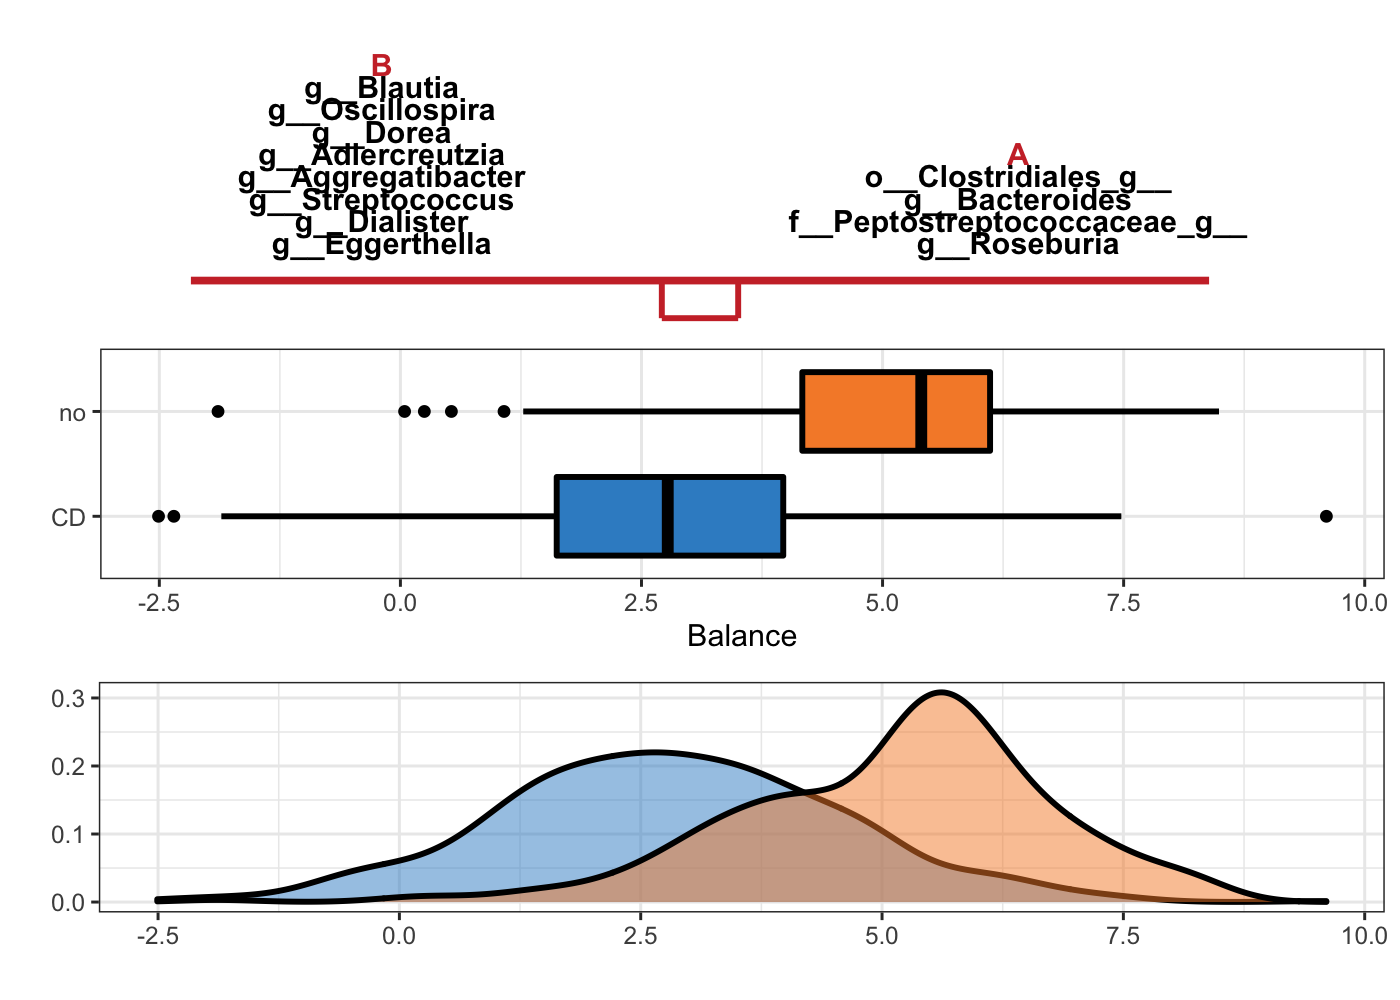
\includegraphics[width=1\linewidth]{./Generated_plots/unnamed-chunk-18-1} \end{center}

\section{HFHS-Day1 case study}\label{hfhs-day1-case-study}

The analysis on HFHSday1 data is similar to Crohn data.

First, we need to check if the dependent variable \textbf{Y} is a
factor.

\begin{Shaded}
\begin{Highlighting}[]
\KeywordTok{class}\NormalTok{(y_HFHSday1)}
\end{Highlighting}
\end{Shaded}

\begin{verbatim}
## [1] "factor"
\end{verbatim}

In HFHSday1 data, we use \emph{selbal\_wrapper()} directly and set the
maximum number of variables to be selected equal to 2 (\textbf{maxV =
2}):

\begin{Shaded}
\begin{Highlighting}[]
\NormalTok{HFHS.results_selbal <-}\StringTok{ }\KeywordTok{selbal_wrapper}\NormalTok{(}\DataTypeTok{X =}\NormalTok{ x_HFHSday1, }\DataTypeTok{Y =}\NormalTok{ y_HFHSday1, }
                                      \DataTypeTok{maxV =} \DecValTok{2}\NormalTok{, }\DataTypeTok{logit.acc =} \StringTok{'Dev'}\NormalTok{) }
\end{Highlighting}
\end{Shaded}

The number of selected variables:

\begin{Shaded}
\begin{Highlighting}[]
\NormalTok{HFHS.results_selbal}\OperatorTok{$}\NormalTok{numVarSelect}
\end{Highlighting}
\end{Shaded}

\begin{verbatim}
## [1] 2
\end{verbatim}

The names of selected variables:

\begin{Shaded}
\begin{Highlighting}[]
\NormalTok{HFHS.results_selbal}\OperatorTok{$}\NormalTok{varSelect}
\end{Highlighting}
\end{Shaded}

\begin{verbatim}
## [1] "290253" "263479"
\end{verbatim}

For visualisation, we then use \emph{selbal\_like\_plot()}.

\begin{Shaded}
\begin{Highlighting}[]
\NormalTok{HFHS.selbal_pos <-}\StringTok{ }\NormalTok{HFHS.results_selbal}\OperatorTok{$}\NormalTok{posVarSelect}
\NormalTok{HFHS.selbal_neg <-}\StringTok{ }\NormalTok{HFHS.results_selbal}\OperatorTok{$}\NormalTok{negVarSelect}
\KeywordTok{selbal_like_plot}\NormalTok{(}\DataTypeTok{pos.names =}\NormalTok{ HFHS.selbal_pos, }\DataTypeTok{neg.names =}\NormalTok{ HFHS.selbal_neg, }
                 \DataTypeTok{Y =}\NormalTok{ y_HFHSday1, }\DataTypeTok{selbal =} \OtherTok{TRUE}\NormalTok{, }
                 \DataTypeTok{FINAL.BAL =}\NormalTok{ HFHS.results_selbal}\OperatorTok{$}\NormalTok{finalBal, }
                 \DataTypeTok{OTU =}\NormalTok{ T, }\DataTypeTok{taxa =}\NormalTok{ taxonomy_HFHS)}
\end{Highlighting}
\end{Shaded}

\begin{center}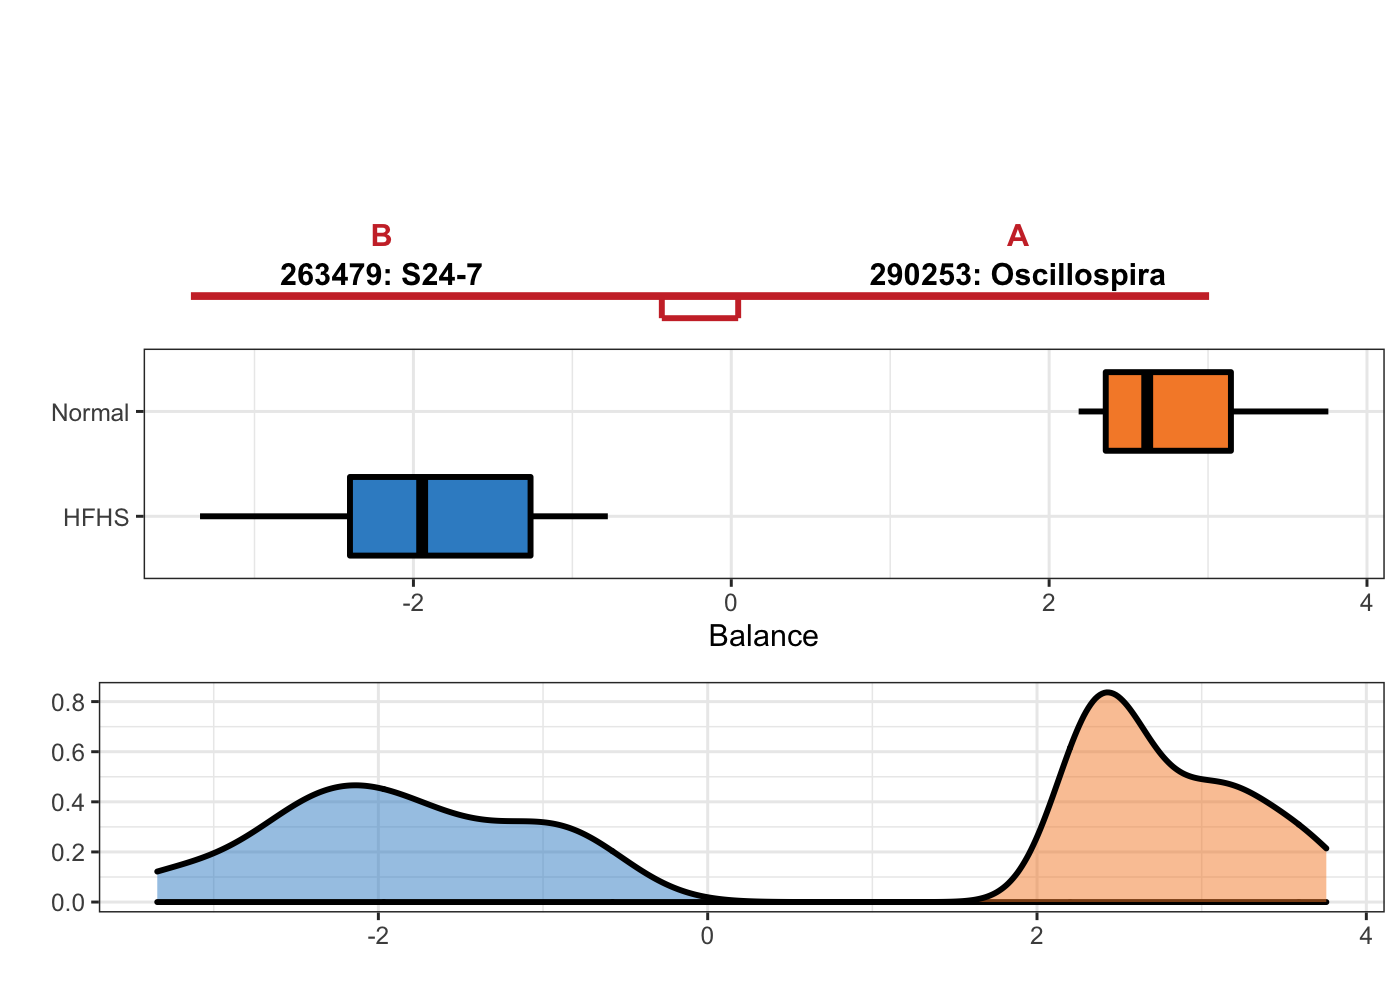
\includegraphics[width=1\linewidth]{./Generated_plots/unnamed-chunk-23-1} \end{center}

We also extract the taxonomic information of these selected OTUs.

\begin{Shaded}
\begin{Highlighting}[]
\NormalTok{HFHS.tax_selbal <-}\StringTok{ }\NormalTok{taxonomy_HFHS[}\KeywordTok{which}\NormalTok{(}\KeywordTok{rownames}\NormalTok{(taxonomy_HFHS) }\OperatorTok\StringTok{ }
\StringTok{                                         }\NormalTok{HFHS.results_selbal}\OperatorTok{$}\NormalTok{varSelect), ]}
\KeywordTok{kable}\NormalTok{(HFHS.tax_selbal[ ,}\DecValTok{2}\OperatorTok{:}\DecValTok{6}\NormalTok{], }\DataTypeTok{booktabs =}\NormalTok{ T)}
\end{Highlighting}
\end{Shaded}

\begin{tabular}{llllll}
\toprule
  & Phylum & Class & Order & Family & Genus\\
\midrule
290253 & Firmicutes & Clostridia & Clostridiales & Ruminococcaceae & Oscillospira\\
263479 & Bacteroidetes & Bacteroidia & Bacteroidales & S24-7 & \\
\bottomrule
\end{tabular}

\chapter{\texorpdfstring{\emph{clr-lasso}}{clr-lasso}}\label{clr}

Penalised regression is a powerful approach for variable selection in
high dimensional settings
\citep{zou2005regularization, tibshirani1996regression, le1992ridge}. It
can be adapted to compositional data analysis (CoDA) by previously
transforming the compositional data with the centered log-ratio
transformation (clr).

\emph{Clr-lasso} implements penalised regression using the R package
\emph{glmnet} after clr transformation. Clr transformation corresponds
to centering the log-transformed values:

\[clr(x) = clr(x_{1},...,x_{k}) = (log(x_{1})-M,...,log(x_{k})-M)\]

Where \(i=1,...,k\) microbial variables, \(x_{k}\) is the counts of
variable \(k\), \(M\) is the arithmetic mean of the log-transformed
values.

\[M = \frac{1}{k}\sum_{i=1}^{k}log(x_{i})\]

We also generated a wrapper function called \emph{glmnet\_wrapper()}
that will call \emph{glmnet()} function within the wrapper and help us
to handle the output of \emph{glmnet}. The \emph{glmnet\_wrapper()}
function is uploaded via \textbf{functions.R}.

\section{Crohn case study}\label{crohn-case-study-1}

First we perform the clr transformation of the abundance table
\textbf{x\_Crohn} as follows (the log-transformation requires a matrix
of positive values and thus the zeros have been previously added with an
offset of 1):

\begin{Shaded}
\begin{Highlighting}[]
\NormalTok{z_Crohn <-}\StringTok{ }\KeywordTok{log}\NormalTok{(x_Crohn)}
\NormalTok{clrx_Crohn <-}\StringTok{ }\KeywordTok{apply}\NormalTok{(z_Crohn, }\DecValTok{2}\NormalTok{, }\ControlFlowTok{function}\NormalTok{(x) x }\OperatorTok{-}\StringTok{ }\KeywordTok{rowMeans}\NormalTok{(z_Crohn))}
\end{Highlighting}
\end{Shaded}

We implement penalised regression with function \emph{glmnet()}. This
function requires the outcome \textbf{Y} to be numeric. The file
``Crohn\_data.RData'' contains \textbf{y\_Crohn\_numeric}, a numerical
vector of disease status with values 1 (CD) and 0 (not CD).

Penalised regression requires the specification of the penalization
parameter \(\lambda\). The larger the value of \(\lambda\), the less
variables will be selected. In previous analysis of this dataset with
\emph{selbal}, a balance with 12 variables was determined optimal to
discriminate the CD status \citep{rivera2018balances}. For ease of
comparison, we will specify the penalisation parameter that results in
the selection of 12 variables for \emph{clr-lasso}.

To identify the value of \(\lambda\) that corresponds to 12 variables
selected we implement \emph{glmnet()} function on the clr transformed
values and with the specification that the response family is
\textbf{binomial}:

\begin{Shaded}
\begin{Highlighting}[]
\NormalTok{Crohn.test_clrlasso <-}\StringTok{ }\KeywordTok{glmnet}\NormalTok{(}\DataTypeTok{x =}\NormalTok{ clrx_Crohn, }\DataTypeTok{y =}\NormalTok{ y_Crohn_numeric, }
                              \DataTypeTok{family =} \StringTok{'binomial'}\NormalTok{, }\DataTypeTok{nlambda =} \DecValTok{30}\NormalTok{)}
\end{Highlighting}
\end{Shaded}

The output of \emph{glmnet()} can be visualised with the selection plot:

\begin{Shaded}
\begin{Highlighting}[]
\KeywordTok{plot}\NormalTok{(Crohn.test_clrlasso, }\DataTypeTok{xvar =} \StringTok{'lambda'}\NormalTok{, }\DataTypeTok{label =}\NormalTok{ T)}
\end{Highlighting}
\end{Shaded}

\begin{figure}

{\centering 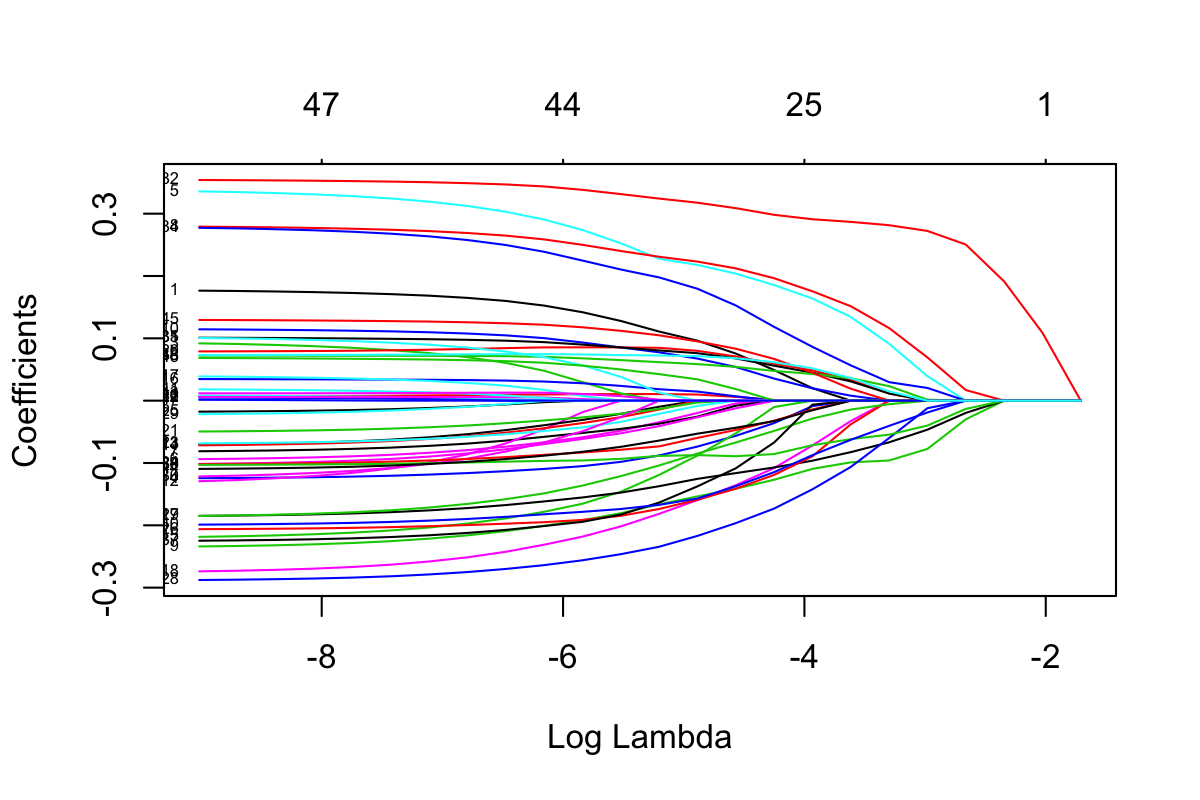
\includegraphics[width=1\linewidth]{./Generated_plots/CDlasso-1} 

}

\caption{Selection plot of Crohn data}\label{fig:CDlasso}
\end{figure}

In Figure \ref{fig:CDlasso}, each curve corresponds to a variable
(i.e.~genus). It shows the path of its coefficient against different
\(log(\lambda)\) values. At each \(log(\lambda)\), the shown curves
indicate the number of nonzero coefficients. In the plot command, if
\textbf{label = T}, each curve will be annotated with variable index.

The numerical output of \emph{glmnet()} will help us to select the value
of \(\lambda\). It provides the number of selected variables or degrees
of freedom of the model (Df), the proportion of explained deviance for a
sequence of values of \(\lambda\):

\begin{Shaded}
\begin{Highlighting}[]
\NormalTok{Crohn.test_clrlasso}
\end{Highlighting}
\end{Shaded}

\begin{verbatim}
## 
## Call:  glmnet(x = clrx_Crohn, y = y_Crohn_numeric, family = "binomial",      nlambda = 30) 
## 
##    Df    %Dev   Lambda
## 1   0 0.00000 0.180900
## 2   1 0.05653 0.131600
## 3   1 0.08761 0.095820
## 4   5 0.12170 0.069750
## 5  10 0.16810 0.050770
## 6  14 0.20670 0.036950
## 7  18 0.24110 0.026900
## 8  23 0.26910 0.019580
## 9  25 0.29220 0.014250
## 10 30 0.30930 0.010370
## 11 32 0.32030 0.007551
## 12 36 0.32770 0.005496
## 13 39 0.33330 0.004001
## 14 41 0.33690 0.002912
## 15 44 0.33910 0.002120
## 16 45 0.34040 0.001543
## 17 46 0.34110 0.001123
## 18 46 0.34150 0.000818
## 19 46 0.34170 0.000595
## 20 47 0.34190 0.000433
## 21 47 0.34190 0.000315
## 22 47 0.34190 0.000230
## 23 47 0.34200 0.000167
## 24 47 0.34200 0.000122
\end{verbatim}

We can see that the value of \(\lambda\) that will select 12 variables
is between 0.037 and 0.051. We perform again \emph{glmnet()} with the
specification of a finer sequence of \(\lambda\) (between 0.03 and 0.05
and an increment of 0.001):

\begin{Shaded}
\begin{Highlighting}[]
\NormalTok{Crohn.test2_clrlasso <-}\StringTok{ }\KeywordTok{glmnet}\NormalTok{(}\DataTypeTok{x =}\NormalTok{ clrx_Crohn, }\DataTypeTok{y =}\NormalTok{ y_Crohn_numeric, }
                               \DataTypeTok{family =} \StringTok{'binomial'}\NormalTok{, }\DataTypeTok{lambda =} \KeywordTok{seq}\NormalTok{(}\FloatTok{0.03}\NormalTok{, }\FloatTok{0.05}\NormalTok{, }\FloatTok{0.001}\NormalTok{))}
\NormalTok{Crohn.test2_clrlasso}
\end{Highlighting}
\end{Shaded}

\begin{verbatim}
## 
## Call:  glmnet(x = clrx_Crohn, y = y_Crohn_numeric, family = "binomial",      lambda = seq(0.03, 0.05, 0.001)) 
## 
##    Df   %Dev Lambda
## 1  10 0.1702  0.050
## 2  10 0.1729  0.049
## 3  10 0.1755  0.048
## 4  10 0.1782  0.047
## 5  11 0.1808  0.046
## 6  11 0.1834  0.045
## 7  11 0.1860  0.044
## 8  12 0.1885  0.043
## 9  13 0.1915  0.042
## 10 14 0.1945  0.041
## 11 14 0.1976  0.040
## 12 14 0.2006  0.039
## 13 14 0.2036  0.038
## 14 14 0.2065  0.037
## 15 14 0.2094  0.036
## 16 14 0.2122  0.035
## 17 14 0.2150  0.034
## 18 15 0.2181  0.033
## 19 18 0.2217  0.032
## 20 18 0.2257  0.031
## 21 18 0.2295  0.030
\end{verbatim}

According to this result, we select \(\lambda = 0.043\) and implement
\emph{glmnet()}:

\begin{Shaded}
\begin{Highlighting}[]
\NormalTok{clrlasso_Crohn <-}\StringTok{ }\KeywordTok{glmnet}\NormalTok{(}\DataTypeTok{x =}\NormalTok{ clrx_Crohn, }\DataTypeTok{y =}\NormalTok{ y_Crohn_numeric, }
                         \DataTypeTok{family =} \StringTok{'binomial'}\NormalTok{, }\DataTypeTok{lambda =} \FloatTok{0.043}\NormalTok{)}
\end{Highlighting}
\end{Shaded}

The same as \emph{selbal}, instead of using the original \emph{glmnet()}
function, we use function \emph{glmnet\_wrapper()} that calls
\emph{glmnet()} function within the wrapper to handle the results of
\emph{clr-lasso} with the same input as \emph{glmnet()}:

\begin{Shaded}
\begin{Highlighting}[]
\NormalTok{Crohn.results_clrlasso <-}\StringTok{ }\KeywordTok{glmnet_wrapper}\NormalTok{(}\DataTypeTok{X =}\NormalTok{ clrx_Crohn, }\DataTypeTok{Y =}\NormalTok{ y_Crohn_numeric, }
                                         \DataTypeTok{family =} \StringTok{'binomial'}\NormalTok{, }\DataTypeTok{lambda =} \FloatTok{0.043}\NormalTok{)}
\end{Highlighting}
\end{Shaded}

We can get the number of selected variables:

\begin{Shaded}
\begin{Highlighting}[]
\NormalTok{Crohn.results_clrlasso}\OperatorTok{$}\NormalTok{numVarSelect}
\end{Highlighting}
\end{Shaded}

\begin{verbatim}
## [1] 12
\end{verbatim}

and the names of the selected variables:

\begin{Shaded}
\begin{Highlighting}[]
\NormalTok{Crohn.results_clrlasso}\OperatorTok{$}\NormalTok{varSelect}
\end{Highlighting}
\end{Shaded}

\begin{verbatim}
##  [1] "g__Roseburia"                 "g__Bacteroides"              
##  [3] "g__Eggerthella"               "f__Peptostreptococcaceae_g__"
##  [5] "g__Dialister"                 "g__Streptococcus"            
##  [7] "g__Adlercreutzia"             "g__Aggregatibacter"          
##  [9] "o__Clostridiales_g__"         "g__Lachnospira"              
## [11] "o__Lactobacillales_g__"       "g__Bilophila"
\end{verbatim}

\section{HFHS-Day1 case study}\label{hfhs-day1-case-study-1}

The analysis on HFHSday1 data is similar to Crohn data. We first perform
the clr transformation:

\begin{Shaded}
\begin{Highlighting}[]
\NormalTok{z_HFHSday1 <-}\StringTok{ }\KeywordTok{log}\NormalTok{(x_HFHSday1)}
\NormalTok{clrx_HFHSday1 <-}\StringTok{ }\KeywordTok{apply}\NormalTok{(z_HFHSday1, }\DecValTok{2}\NormalTok{, }\ControlFlowTok{function}\NormalTok{(x) x}\OperatorTok{-}\KeywordTok{rowMeans}\NormalTok{(z_HFHSday1))}
\end{Highlighting}
\end{Shaded}

The outcome \textbf{y\_HFHSday1} is converted to a numeric vector.

\begin{Shaded}
\begin{Highlighting}[]
\NormalTok{y_HFHSday1_numeric <-}\StringTok{ }\KeywordTok{as.numeric}\NormalTok{(y_HFHSday1)}
\end{Highlighting}
\end{Shaded}

We implement \emph{glmnet()} and visualise the results (Figure
\ref{fig:HFHSlasso}).

\begin{Shaded}
\begin{Highlighting}[]
\NormalTok{HFHS.test_clrlasso <-}\StringTok{ }\KeywordTok{glmnet}\NormalTok{(}\DataTypeTok{x =}\NormalTok{ clrx_HFHSday1, }\DataTypeTok{y =}\NormalTok{ y_HFHSday1_numeric, }
                             \DataTypeTok{family =} \StringTok{'binomial'}\NormalTok{, }\DataTypeTok{nlambda =} \DecValTok{30}\NormalTok{)}
\end{Highlighting}
\end{Shaded}

\begin{Shaded}
\begin{Highlighting}[]
\KeywordTok{plot}\NormalTok{(HFHS.test_clrlasso, }\DataTypeTok{xvar =} \StringTok{'lambda'}\NormalTok{, }\DataTypeTok{label =}\NormalTok{ T)}
\end{Highlighting}
\end{Shaded}

\begin{figure}

{\centering 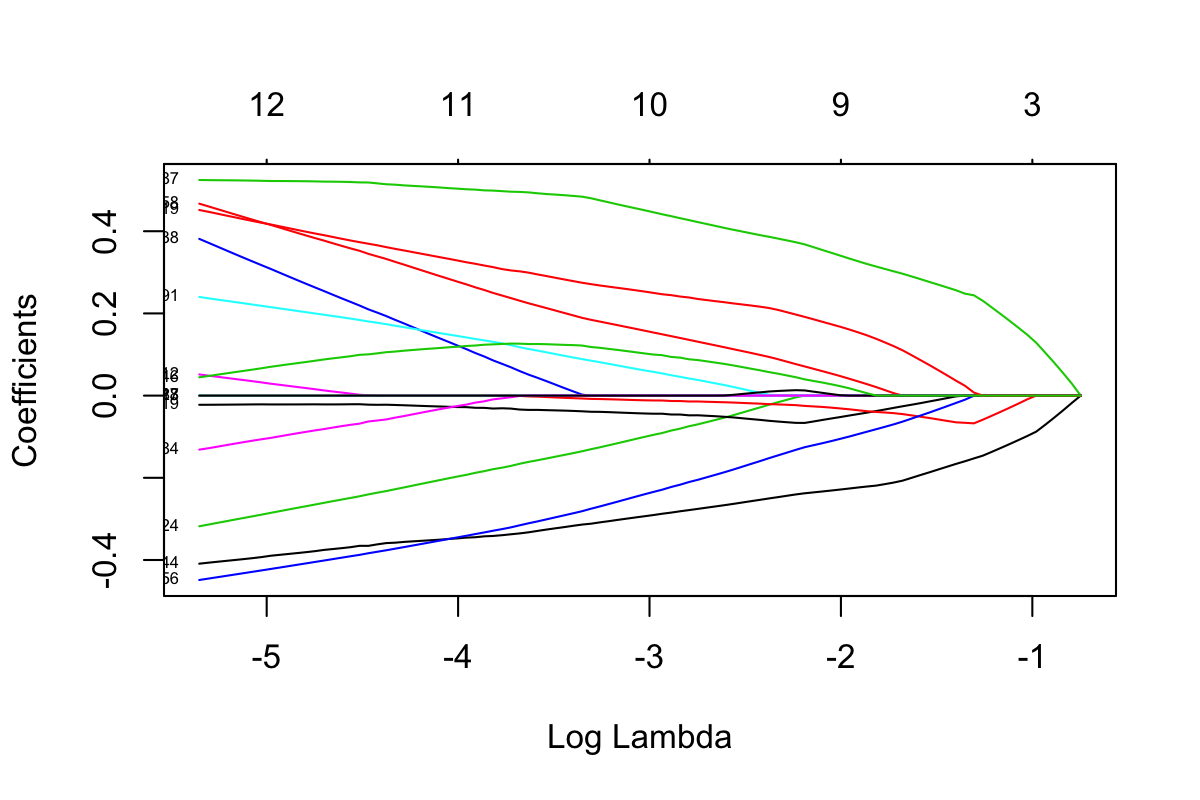
\includegraphics[width=1\linewidth]{./Generated_plots/HFHSlasso-1} 

}

\caption{Lasso plot of HFHS-Day1 data}\label{fig:HFHSlasso}
\end{figure}

The explanation of Figure \ref{fig:HFHSlasso} is the same as Figure
\ref{fig:CDlasso}.

The numerical output of \emph{glmnet()} will help us to decide the
penalty term \(\lambda\):

\begin{Shaded}
\begin{Highlighting}[]
\NormalTok{HFHS.test_clrlasso}
\end{Highlighting}
\end{Shaded}

\begin{verbatim}
## 
## Call:  glmnet(x = clrx_HFHSday1, y = y_HFHSday1_numeric, family = "binomial",      nlambda = 30) 
## 
##    Df   %Dev  Lambda
## 1   0 0.0000 0.47370
## 2   2 0.1862 0.40420
## 3   3 0.3290 0.34480
## 4   3 0.4417 0.29420
## 5   6 0.5335 0.25100
## 6   6 0.6089 0.21410
## 7   7 0.6707 0.18270
## 8   8 0.7221 0.15590
## 9   9 0.7649 0.13300
## 10  9 0.8007 0.11350
## 11 11 0.8309 0.09680
## 12 11 0.8564 0.08259
## 13 10 0.8778 0.07046
## 14 10 0.8959 0.06011
## 15 10 0.9113 0.05129
## 16 10 0.9244 0.04376
## 17 10 0.9354 0.03733
## 18 11 0.9449 0.03185
## 19 10 0.9530 0.02717
## 20 11 0.9599 0.02318
## 21 11 0.9657 0.01978
## 22 11 0.9707 0.01688
## 23 11 0.9750 0.01440
## 24 12 0.9786 0.01228
## 25 12 0.9818 0.01048
## 26 12 0.9844 0.00894
## 27 12 0.9867 0.00763
## 28 12 0.9886 0.00651
## 29 12 0.9903 0.00555
## 30 13 0.9917 0.00474
\end{verbatim}

For comparison purposes we set the penalty term \(\lambda\) equal to
0.03 that results in the selection of 10 OTUs. In HFHSday1 data, we use
\emph{glmnet\_wrapper()} directly and set the extra input
\textbf{\(\lambda = 0.03\)}:

\begin{Shaded}
\begin{Highlighting}[]
\NormalTok{HFHS.results_clrlasso <-}\StringTok{ }\KeywordTok{glmnet_wrapper}\NormalTok{(}\DataTypeTok{X =}\NormalTok{ clrx_HFHSday1, }\DataTypeTok{Y =}\NormalTok{ y_HFHSday1_numeric, }
                                        \DataTypeTok{family =} \StringTok{'binomial'}\NormalTok{, }\DataTypeTok{lambda =} \FloatTok{0.03}\NormalTok{) }
\end{Highlighting}
\end{Shaded}

Then we get the number of selected variables:

\begin{Shaded}
\begin{Highlighting}[]
\NormalTok{HFHS.results_clrlasso}\OperatorTok{$}\NormalTok{numVarSelect}
\end{Highlighting}
\end{Shaded}

\begin{verbatim}
## [1] 10
\end{verbatim}

and the names of selected variables:

\begin{Shaded}
\begin{Highlighting}[]
\NormalTok{HFHS.results_clrlasso}\OperatorTok{$}\NormalTok{varSelect}
\end{Highlighting}
\end{Shaded}

\begin{verbatim}
##  [1] "400599"  "192222"  "348038"  "401384"  "290253"  "261265"  "300851" 
##  [8] "462764"  "1108745" "265322"
\end{verbatim}

We also extract the taxonomic information of these selected OTUs.

\begin{Shaded}
\begin{Highlighting}[]
\NormalTok{HFHS.tax_clrlasso <-}\StringTok{ }\NormalTok{taxonomy_HFHS[}\KeywordTok{which}\NormalTok{(}\KeywordTok{rownames}\NormalTok{(taxonomy_HFHS) }\OperatorTok\StringTok{ }
\StringTok{                                           }\NormalTok{HFHS.results_clrlasso}\OperatorTok{$}\NormalTok{varSelect), ]}
\KeywordTok{kable}\NormalTok{(HFHS.tax_clrlasso[ ,}\DecValTok{2}\OperatorTok{:}\DecValTok{6}\NormalTok{], }\DataTypeTok{booktabs =}\NormalTok{ T)}
\end{Highlighting}
\end{Shaded}

\begin{tabular}{llllll}
\toprule
  & Phylum & Class & Order & Family & Genus\\
\midrule
192222 & Bacteroidetes & Bacteroidia & Bacteroidales & Prevotellaceae & \\
290253 & Firmicutes & Clostridia & Clostridiales & Ruminococcaceae & Oscillospira\\
261265 & Firmicutes & Clostridia & Clostridiales & Lachnospiraceae & \\
1108745 & Firmicutes & Clostridia & Clostridiales & [Mogibacteriaceae] & \\
462764 & Firmicutes & Clostridia & Clostridiales & Ruminococcaceae & Ruminococcus\\
\addlinespace
265322 & Bacteroidetes & Bacteroidia & Bacteroidales & S24-7 & \\
400599 & Firmicutes & Clostridia & Clostridiales &  & \\
348038 & Bacteroidetes & Bacteroidia & Bacteroidales & S24-7 & \\
401384 & Firmicutes & Clostridia & Clostridiales & Ruminococcaceae & Oscillospira\\
300851 & Firmicutes & Clostridia & Clostridiales & Ruminococcaceae & Oscillospira\\
\bottomrule
\end{tabular}

\chapter{\texorpdfstring{\emph{coda-lasso}}{coda-lasso}}\label{coda}

\emph{Coda-lasso} implements penalised regression on a log-contrast
model (a regression model on log-transformed covariates and a zero-sum
constraint on the regression coefficients, except the intercept)
\citep{lu2019generalized, lin2014variable}.

As we mentioned before, \emph{coda-lasso} is not yet available as an R
package. Our R code for implementing the algorithm includes two main
functions that are \emph{coda\_logistic\_lasso()} and
\emph{coda\_logistic\_elasticNet()} that implement LASSO or elastic-net
penalisation on a logistic regression model for a binary outcome.

Details of function
\emph{coda\_logistic\_lasso}(\textbf{y},\textbf{X},\textbf{lambda}):

\textbf{y} is the binary outcome, can be numerical (values 0 and 1),
factor (2 levels) or categorical (2 categories).

\textbf{X} is the matrix of microbiome abundances, either absolute
abundances (counts) or relative abundances (proportions), the rows of
\textbf{X} are individuals/samples, the columns are taxa.

\textbf{lambda} is the penalisation parameter, the larger the value of
\textbf{lambda} the smaller the number of variables selected.

\emph{Notes}:

\begin{itemize}
\tightlist
\item
  Imputation of zeros: The user should provide a matrix \textbf{X} of
  positive values without zeros. Zeros should be previously added with
  an offset of 1 by the user.
\item
  Log-transformation: \textbf{X} should not be the matrix of log(counts)
  or log(proportions). The method itself performs the log-transformation
  of the abundances.
\item
  Selection of \(\lambda\): Functions \emph{lambdaRange\_codalasso()}
  and \emph{lambdaRange\_elasticnet()} are useful to find the optimum
  value of the penalisation parameter \(\lambda\). Function
  \emph{lambdaRange\_codalasso}(\textbf{y},\textbf{X}) provides the
  number of selected variables and the proportion of explained deviance
  for a sequence of values for the penalised parameter \(\lambda\).
\end{itemize}

Bellow, we illustrate the use of \emph{coda\_logistic\_lasso()} on the
Crohn and HFHS-Day1 case studies. We also generated a wrapper function
called \emph{coda\_lasso\_wrapper()} that will call
\emph{coda\_logistic\_lasso()} function within the wrapper and help us
to handle the output of \emph{coda-lasso}. The
\emph{coda\_lasso\_wrapper()} function is uploaded via
\textbf{functions.R}.

\section{Crohn case study}\label{crohn-case-study-2}

To run \emph{coda-lasso}, we must specify a value of \(\lambda\), the
penalisation parameter: the larger the value of \(\lambda\), the less
variables will be selected. In previous analysis of this dataset with
\emph{selbal}, a balance with 12 variables was determined optimal to
discriminate the CD status \citep{rivera2018balances}. For ease of
comparison, we will specify the penalised parameter that results in the
selection of 12 variables for \emph{coda-lasso}. Function
\emph{lambdaRange\_codalasso()} helps us to identify the value of
\(\lambda\) that corresponds to 12 variables selected. To save space, we
only consider a sequence of \(\lambda\) from 0.1 to 0.2 with an
increment of 0.01, but you can start from a broader range:

\begin{Shaded}
\begin{Highlighting}[]
\KeywordTok{lambdaRange_codalasso}\NormalTok{(}\DataTypeTok{X =}\NormalTok{ x_Crohn, }\DataTypeTok{y =}\NormalTok{ y_Crohn, }\DataTypeTok{lambdaSeq =} \KeywordTok{seq}\NormalTok{(}\FloatTok{0.1}\NormalTok{, }\FloatTok{0.2}\NormalTok{, }\FloatTok{0.01}\NormalTok{))}
\end{Highlighting}
\end{Shaded}

\begin{verbatim}
## [1] "lambda"             "num.selected"       "prop.explained.dev"
## 0.1000  23  0.2473
## 0.1100  18  0.2398
## 0.1200  17  0.2355
## 0.1300  25  0.2288
## 0.1400  13  0.2185
## 0.1500  12  0.2130
## 0.1600  12  0.2043
## 0.1700  14  0.2010
## 0.1800  11  0.1908
## 0.1900  10  0.1903
## 0.2000  8  0.1775
\end{verbatim}

In this output, the first column is the value of \(\lambda\), the second
column is the number of selected variables and the third column is the
proportion of deviance explained. According to this results, we will
take \(\lambda = 0.15\).

\begin{Shaded}
\begin{Highlighting}[]
\NormalTok{codalasso_Crohn <-}\StringTok{ }\KeywordTok{coda_logistic_lasso}\NormalTok{(}\DataTypeTok{X =}\NormalTok{ x_Crohn, }\DataTypeTok{y =}\NormalTok{ y_Crohn, }\DataTypeTok{lambda =} \FloatTok{0.15}\NormalTok{)}
\end{Highlighting}
\end{Shaded}

The same as the previous two methods, we also use a wrapper function
called \emph{coda\_lasso\_wrapper()} instead of the original
\emph{coda\_logistic\_lasso()} function. This wrapper function calls
\emph{coda\_logistic\_lasso()} function within the wrapper and with the
same input as \emph{coda\_logistic\_lasso()}.

\begin{Shaded}
\begin{Highlighting}[]
\NormalTok{Crohn.results_codalasso <-}\StringTok{ }\KeywordTok{coda_lasso_wrapper}\NormalTok{(}\DataTypeTok{X =}\NormalTok{ x_Crohn, }\DataTypeTok{Y =}\NormalTok{ y_Crohn, }
                                              \DataTypeTok{lambda =} \FloatTok{0.15}\NormalTok{)}
\end{Highlighting}
\end{Shaded}

Then we get the number of selected variables:

\begin{Shaded}
\begin{Highlighting}[]
\NormalTok{Crohn.results_codalasso}\OperatorTok{$}\NormalTok{numVarSelect}
\end{Highlighting}
\end{Shaded}

\begin{verbatim}
## [1] 12
\end{verbatim}

and the names of selected variables:

\begin{Shaded}
\begin{Highlighting}[]
\NormalTok{Crohn.results_codalasso}\OperatorTok{$}\NormalTok{varSelect}
\end{Highlighting}
\end{Shaded}

\begin{verbatim}
##  [1] "g__Roseburia"                 "g__Streptococcus"            
##  [3] "g__Dialister"                 "f__Peptostreptococcaceae_g__"
##  [5] "g__Aggregatibacter"           "g__Eggerthella"              
##  [7] "g__Prevotella"                "g__Dorea"                    
##  [9] "g__Bilophila"                 "o__Lactobacillales_g__"      
## [11] "g__Lachnospira"               "g__Clostridium"
\end{verbatim}

\section{HFHS-Day1 case study}\label{hfhs-day1-case-study-2}

The analysis on HFHSday1 data is similar to Crohn data.

Using function \emph{lambdaRange\_codalasso()}, we explore the number of
selected OTUs and the proportion of explained variance for different
values of \(\lambda\). To save space, we only consider a sequence of
\(\lambda\) from 1.3 to 1.8 with an increment of 0.01, but you can start
from a broader range:

\begin{Shaded}
\begin{Highlighting}[]
\KeywordTok{lambdaRange_codalasso}\NormalTok{(}\DataTypeTok{X =}\NormalTok{ x_HFHSday1, }\DataTypeTok{y =}\NormalTok{ y_HFHSday1, }\DataTypeTok{lambdaSeq =} \KeywordTok{seq}\NormalTok{(}\FloatTok{1.3}\NormalTok{, }\FloatTok{1.8}\NormalTok{, }\FloatTok{0.01}\NormalTok{))}
\end{Highlighting}
\end{Shaded}

\begin{verbatim}
## [1] "lambda"             "num.selected"       "prop.explained.dev"
## 1.3000  8  1.0000
## 1.3100  8  1.0000
## 1.3200  8  1.0000
## 1.3300  8  1.0000
## 1.3400  8  1.0000
## 1.3500  8  1.0000
## 1.3600  8  1.0000
## 1.3700  8  1.0000
## 1.3800  9  1.0000
## 1.3900  9  1.0000
## 1.4000  9  1.0000
## 1.4100  9  1.0000
## 1.4200  9  1.0000
## 1.4300  9  1.0000
## 1.4400  7  1.0000
## 1.4500  7  1.0000
## 1.4600  7  1.0000
## 1.4700  7  1.0000
## 1.4800  6  0.6344
## 1.4900  6  0.6344
## 1.5000  6  0.6344
## 1.5100  6  0.6343
## 1.5200  6  0.6343
## 1.5300  6  0.6343
## 1.5400  6  0.6343
## 1.5500  6  0.6343
## 1.5600  6  0.6342
## 1.5700  3  0.0108
## 1.5800  3  0.0089
## 1.5900  3  0.0130
## 1.6000  3  0.0241
## 1.6100  3  0.0290
## 1.6200  3  0.0441
## 1.6300  3  0.0481
## 1.6400  3  0.0644
## 1.6500  3  0.0667
## 1.6600  3  0.0688
## 1.6700  3  0.0700
## 1.6800  3  0.0822
## 1.6900  3  0.0829
## 1.7000  3  0.0835
## 1.7100  3  0.0841
## 1.7200  3  0.0847
## 1.7300  3  0.0854
## 1.7400  3  0.0860
## 1.7500  3  0.0866
## 1.7600  3  0.0872
## 1.7700  3  0.0878
## 1.7800  3  0.0884
## 1.7900  3  0.0890
## 1.8000  3  0.0895
\end{verbatim}

The largest \(\lambda\) that provides maximum proportion of explained
deviance is \(\lambda = 1.47\). Thus, we implement \emph{coda-lasso}
with this value of \(\lambda\).

In HFHSday1 data, we use \emph{coda\_lasso\_wrapper()} directly.

\begin{Shaded}
\begin{Highlighting}[]
\NormalTok{HFHS.results_codalasso <-}\StringTok{ }\KeywordTok{coda_lasso_wrapper}\NormalTok{(}\DataTypeTok{X =}\NormalTok{ x_HFHSday1, }\DataTypeTok{Y =}\NormalTok{ y_HFHSday1, }\DataTypeTok{lambda =} \FloatTok{1.47}\NormalTok{) }
\end{Highlighting}
\end{Shaded}

The number of selected variables is 7:

\begin{Shaded}
\begin{Highlighting}[]
\NormalTok{HFHS.results_codalasso}\OperatorTok{$}\NormalTok{numVarSelect}
\end{Highlighting}
\end{Shaded}

\begin{verbatim}
## [1] 7
\end{verbatim}

The proportion of explained deviance by the selected OTUs is 1 meaning
that they completely discriminate the two diet groups:

\begin{Shaded}
\begin{Highlighting}[]
\NormalTok{HFHS.results_codalasso}\OperatorTok{$}\NormalTok{explained_deviance_proportion}
\end{Highlighting}
\end{Shaded}

\begin{verbatim}
## [1] 1
\end{verbatim}

The names of the selected OTUs are:

\begin{Shaded}
\begin{Highlighting}[]
\NormalTok{HFHS.results_codalasso}\OperatorTok{$}\NormalTok{varSelect}
\end{Highlighting}
\end{Shaded}

\begin{verbatim}
## [1] "348038" "400599" "192222" "198339" "265322" "263479" "175272"
\end{verbatim}

By using the taxomonic table, we extract the taxonomic information of
these selected OTUs.

\begin{Shaded}
\begin{Highlighting}[]
\NormalTok{HFHS.tax_codalasso <-}\StringTok{ }\NormalTok{taxonomy_HFHS[}\KeywordTok{which}\NormalTok{(}\KeywordTok{rownames}\NormalTok{(taxonomy_HFHS) }\OperatorTok\StringTok{ }
\StringTok{                                            }\NormalTok{HFHS.results_codalasso}\OperatorTok{$}\NormalTok{varSelect), ]}
\KeywordTok{kable}\NormalTok{(HFHS.tax_codalasso[ ,}\DecValTok{2}\OperatorTok{:}\DecValTok{6}\NormalTok{], }\DataTypeTok{booktabs =}\NormalTok{ T)}
\end{Highlighting}
\end{Shaded}

\begin{tabular}{llllll}
\toprule
  & Phylum & Class & Order & Family & Genus\\
\midrule
192222 & Bacteroidetes & Bacteroidia & Bacteroidales & Prevotellaceae & \\
265322 & Bacteroidetes & Bacteroidia & Bacteroidales & S24-7 & \\
263479 & Bacteroidetes & Bacteroidia & Bacteroidales & S24-7 & \\
400599 & Firmicutes & Clostridia & Clostridiales &  & \\
348038 & Bacteroidetes & Bacteroidia & Bacteroidales & S24-7 & \\
\addlinespace
198339 & Bacteroidetes & Bacteroidia & Bacteroidales & S24-7 & \\
175272 & Bacteroidetes & Bacteroidia & Bacteroidales & S24-7 & \\
\bottomrule
\end{tabular}

\chapter{Concordance of variables selected by the three
methods}\label{comparison}

In this chapter, we are going to use different visualisation approaches
to display the variables selected by the three methods:

\begin{itemize}
\tightlist
\item
  \emph{UpSet plot}: highlights overlap of the variables selected by the
  three methods.
\item
  \emph{Selbal-like plot}: lists the selected variables and displays
  their discriminating ability with respect to sample groups.
\item
  \emph{plotLoadings}: visualises the variable coefficients and sample
  groups each variable contributes to.
\item
  \emph{Trajectory plot}: represents the rank of the variables selected
  by \emph{coda-lasso} and \emph{clr-lasso}, and their corresponding
  regression coefficients
\item
  \emph{GraPhlAn}: displays the taxonomic tree of selected variables
  (HFHSday1 data only).
\end{itemize}

\section{Crohn case study}\label{crohn-case-study-3}

\subsection{UpSetR}\label{upsetr}

\emph{UpSet} is a visualisation technique for the quantitative analysis
of sets and their intersections \citep{lex2014upset}. Before we apply
\emph{upset()}, we take the list of variable vectors selected with the
three methods and convert them into a data frame compatible with
\emph{upset()} using \emph{fromList()}. We then assign different color
shcemes for each variable selection.

\begin{Shaded}
\begin{Highlighting}[]
\NormalTok{Crohn.select <-}\StringTok{ }\KeywordTok{list}\NormalTok{(}\DataTypeTok{selbal =}\NormalTok{ Crohn.results_selbal}\OperatorTok{$}\NormalTok{varSelect,}
                     \DataTypeTok{clr_lasso =}\NormalTok{ Crohn.results_clrlasso}\OperatorTok{$}\NormalTok{varSelect,}
                     \DataTypeTok{coda_lasso =}\NormalTok{ Crohn.results_codalasso}\OperatorTok{$}\NormalTok{varSelect)}


\NormalTok{Crohn.select.upsetR <-}\StringTok{ }\KeywordTok{fromList}\NormalTok{(Crohn.select)}

\KeywordTok{upset}\NormalTok{(}\KeywordTok{as.data.frame}\NormalTok{(Crohn.select.upsetR), }\DataTypeTok{main.bar.color =} \StringTok{'gray36'}\NormalTok{, }
      \DataTypeTok{sets.bar.color =}\NormalTok{ color[}\KeywordTok{c}\NormalTok{(}\DecValTok{1}\OperatorTok{:}\DecValTok{2}\NormalTok{,}\DecValTok{5}\NormalTok{)], }\DataTypeTok{matrix.color =} \StringTok{'gray36'}\NormalTok{, }
      \DataTypeTok{order.by =} \StringTok{'freq'}\NormalTok{, }\DataTypeTok{empty.intersections =} \StringTok{'on'}\NormalTok{, }
      \DataTypeTok{queries =} \KeywordTok{list}\NormalTok{(}\KeywordTok{list}\NormalTok{(}\DataTypeTok{query =}\NormalTok{ intersects, }\DataTypeTok{params =} \KeywordTok{list}\NormalTok{(}\StringTok{'selbal'}\NormalTok{), }
                          \DataTypeTok{color =}\NormalTok{ color[}\DecValTok{5}\NormalTok{], }\DataTypeTok{active =}\NormalTok{ T), }
                     \KeywordTok{list}\NormalTok{(}\DataTypeTok{query =}\NormalTok{ intersects, }\DataTypeTok{params =} \KeywordTok{list}\NormalTok{(}\StringTok{'clr_lasso'}\NormalTok{), }
                          \DataTypeTok{color =}\NormalTok{ color[}\DecValTok{2}\NormalTok{], }\DataTypeTok{active =}\NormalTok{ T),}
                     \KeywordTok{list}\NormalTok{(}\DataTypeTok{query =}\NormalTok{ intersects, }\DataTypeTok{params =} \KeywordTok{list}\NormalTok{(}\StringTok{'coda_lasso'}\NormalTok{), }
                          \DataTypeTok{color =}\NormalTok{ color[}\DecValTok{1}\NormalTok{], }\DataTypeTok{active =}\NormalTok{ T)))}
\end{Highlighting}
\end{Shaded}

\begin{figure}

{\centering 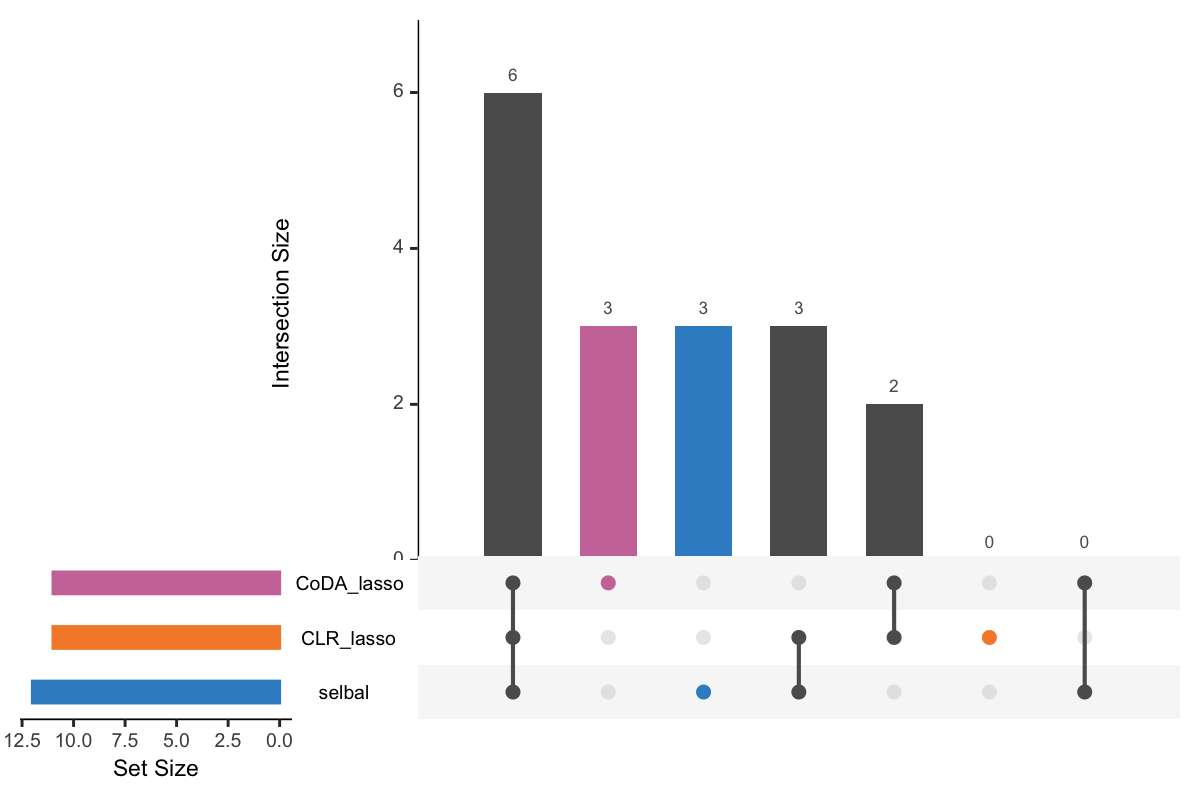
\includegraphics[width=1\linewidth]{./Generated_plots/upsetCD-1} 

}

\caption{UpSet plot showing overlap between variables selected with different methods.}\label{fig:upsetCD}
\end{figure}

In Figure \ref{fig:upsetCD}, the left bars show the number of variables
selected by each method. The right bar plot combined with the
scatterplot show different intersection and their aggregates. For
example, in the first column, three points are linked with one line, and
the intersection size of the bar is 6. This means that 6 variables are
selected by all these three methods. While in the second column, 3
variables are only selected by the method \emph{selbal} and
\emph{clr-lasso}.

\subsection{Selbal-like plot}\label{selbal-like-plot}

As mentioned in Chapter \ref{selbal}, \emph{selbal} visualised the
results using a mixture of selected variables, box plots and density
plots:

\begin{Shaded}
\begin{Highlighting}[]
\CommentTok{# selbal}
\NormalTok{Crohn.selbal_pos <-}\StringTok{ }\NormalTok{Crohn.results_selbal}\OperatorTok{$}\NormalTok{posVarSelect}
\NormalTok{Crohn.selbal_neg <-}\StringTok{ }\NormalTok{Crohn.results_selbal}\OperatorTok{$}\NormalTok{negVarSelect}
\KeywordTok{selbal_like_plot}\NormalTok{(}\DataTypeTok{pos.names =}\NormalTok{ Crohn.selbal_pos, }
                 \DataTypeTok{neg.names =}\NormalTok{ Crohn.selbal_neg, }
                 \DataTypeTok{Y =}\NormalTok{ y_Crohn, }\DataTypeTok{selbal =} \OtherTok{TRUE}\NormalTok{, }
                 \DataTypeTok{FINAL.BAL =}\NormalTok{ Crohn.results_selbal}\OperatorTok{$}\NormalTok{finalBal)}
\end{Highlighting}
\end{Shaded}

\begin{figure}

{\centering 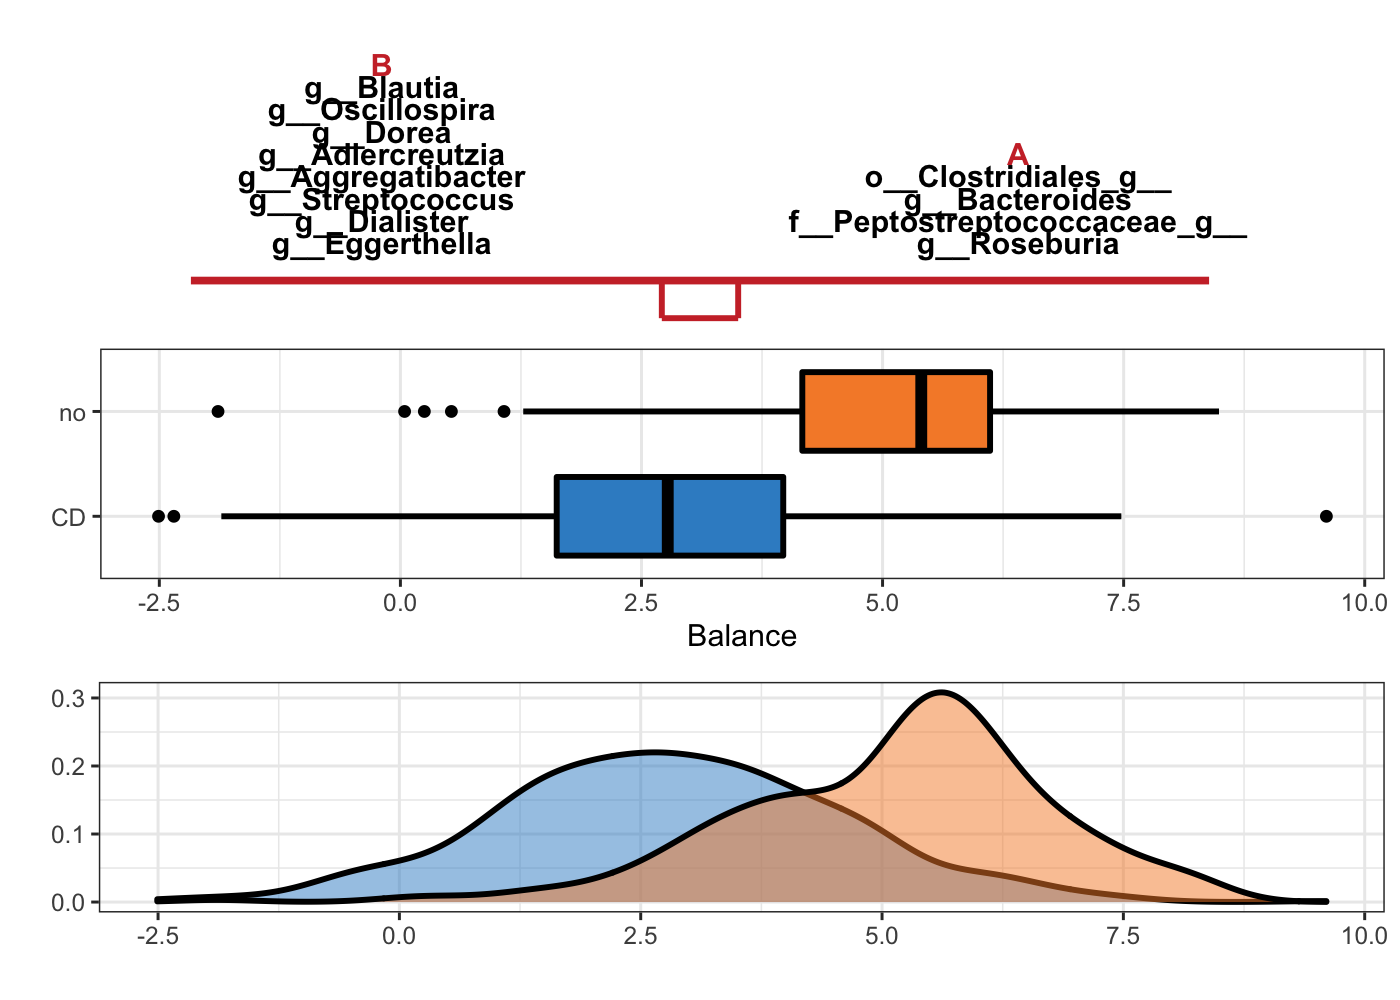
\includegraphics[width=1\linewidth]{./Generated_plots/selbalCD-1} 

}

\caption{Selbal plot showing variables selected with method selbal and the ability of these variables to discriminate CD and non-CD individuals.}\label{fig:selbalCD}
\end{figure}

In Figure \ref{fig:selbalCD}, the two groups of variables that form the
global balance are specified at the top of the plot. They are equally
important. The middle box plots represent the distribution of the
balance scores for CD and non-CD individuals. The bottom part of the
figure contains the density curve for each group.

\emph{Selbal-like plot} is an extension of this kind of plots. Besides
the visualisation of \emph{selbal}, it can also be used to visualise the
results from \emph{clr-lasso} and \emph{coda-lasso}, and generate
similar plots as Figure \ref{fig:selbalCD}.

\begin{Shaded}
\begin{Highlighting}[]
\CommentTok{# clr_lasso}
\NormalTok{Crohn.clr_pos <-}\StringTok{ }\NormalTok{Crohn.results_clrlasso}\OperatorTok{$}\NormalTok{posCoefSelect}
\NormalTok{Crohn.clr_neg <-}\StringTok{ }\NormalTok{Crohn.results_clrlasso}\OperatorTok{$}\NormalTok{negCoefSelect}
\KeywordTok{selbal_like_plot}\NormalTok{(}\DataTypeTok{pos.names =} \KeywordTok{names}\NormalTok{(Crohn.clr_pos), }
                 \DataTypeTok{neg.names =} \KeywordTok{names}\NormalTok{(Crohn.clr_neg), }
                 \DataTypeTok{Y =}\NormalTok{ y_Crohn, }\DataTypeTok{X =}\NormalTok{ x_Crohn)}
\end{Highlighting}
\end{Shaded}

\begin{figure}

{\centering 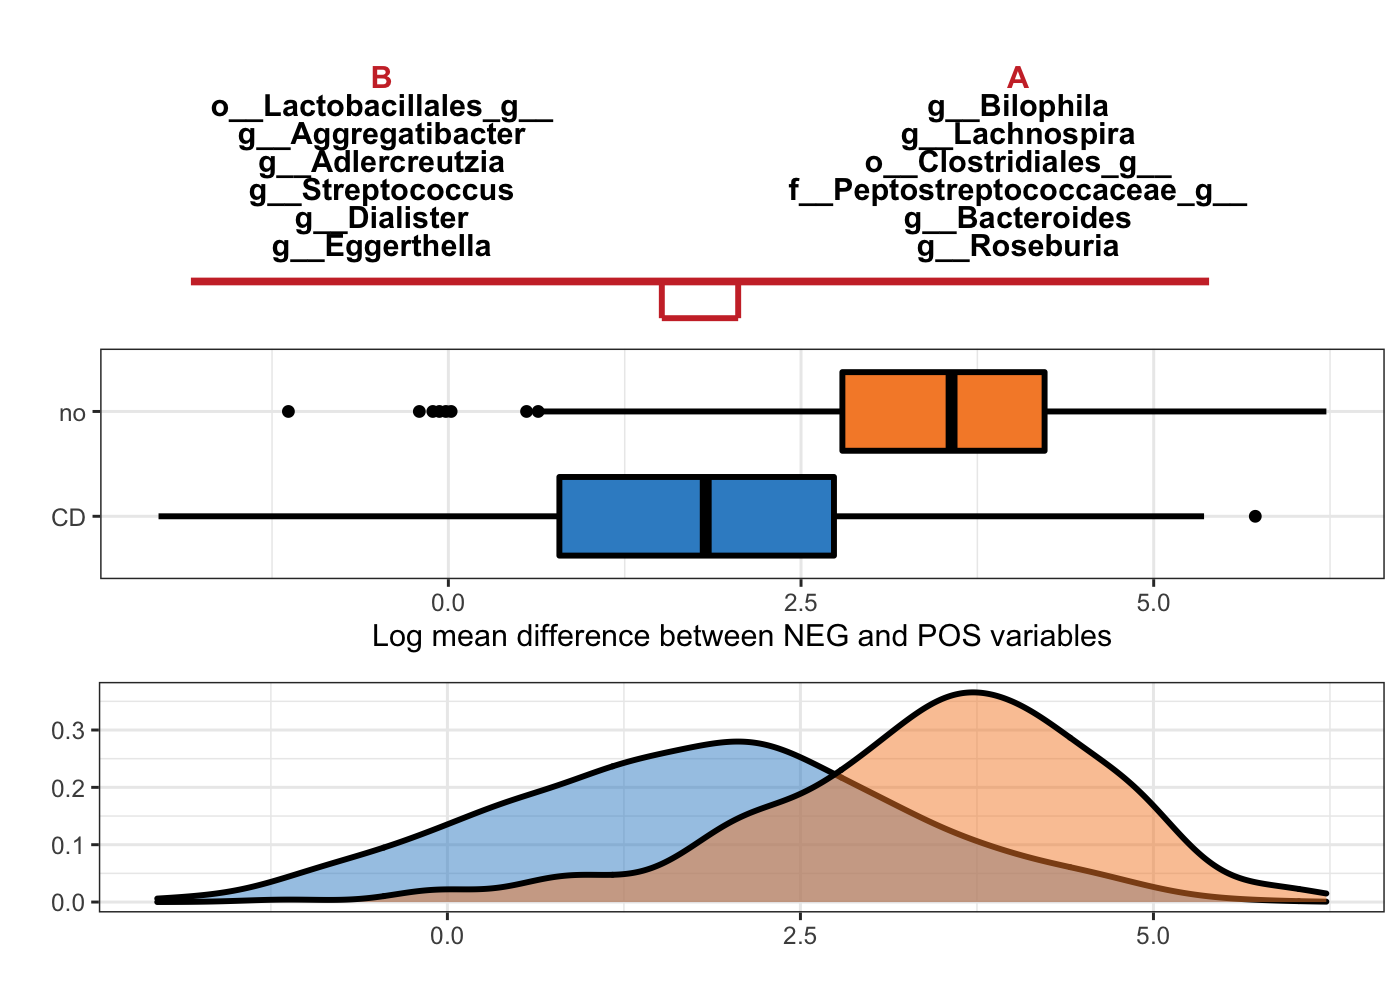
\includegraphics[width=1\linewidth]{./Generated_plots/clrCD-1} 

}

\caption{Selbal-like plot showing variables selected with method clr-lasso and the ability of these variables to discriminate CD and non-CD individuals.}\label{fig:clrCD}
\end{figure}

In Figure \ref{fig:clrCD}, the top panel lists the selected variable
names with either negative (B) or positive (A) coefficients. The names
are ordered according to their importance (absolute coefficient values).
The middle boxplots are based on the log mean difference between
negative and positive variables:
\(\frac{1}{p_{+}}\sum_{i=1}^{p_{+}}logX_{i} - \frac{1}{p_{-}}\sum_{j=1}^{p_{-}}logX_{j}\).
This log mean difference is calculated for each sample as a balance
score, because it is proportionally equal to the balance mentioned in
\citep{rivera2018balances}. The bottom density plots represent the
distributions of the log mean difference scores for CD and non-CD
individuals.

\begin{Shaded}
\begin{Highlighting}[]
\CommentTok{# coda_lasso}
\NormalTok{Crohn.coda_pos <-}\StringTok{ }\NormalTok{Crohn.results_codalasso}\OperatorTok{$}\NormalTok{posCoefSelect}
\NormalTok{Crohn.coda_neg <-}\StringTok{ }\NormalTok{Crohn.results_codalasso}\OperatorTok{$}\NormalTok{negCoefSelect}
\KeywordTok{selbal_like_plot}\NormalTok{(}\DataTypeTok{pos.names =} \KeywordTok{names}\NormalTok{(Crohn.coda_pos), }
                 \DataTypeTok{neg.names =} \KeywordTok{names}\NormalTok{(Crohn.coda_neg), }
                 \DataTypeTok{Y =}\NormalTok{ y_Crohn, }\DataTypeTok{X =}\NormalTok{ x_Crohn)}
\end{Highlighting}
\end{Shaded}

\begin{figure}

{\centering 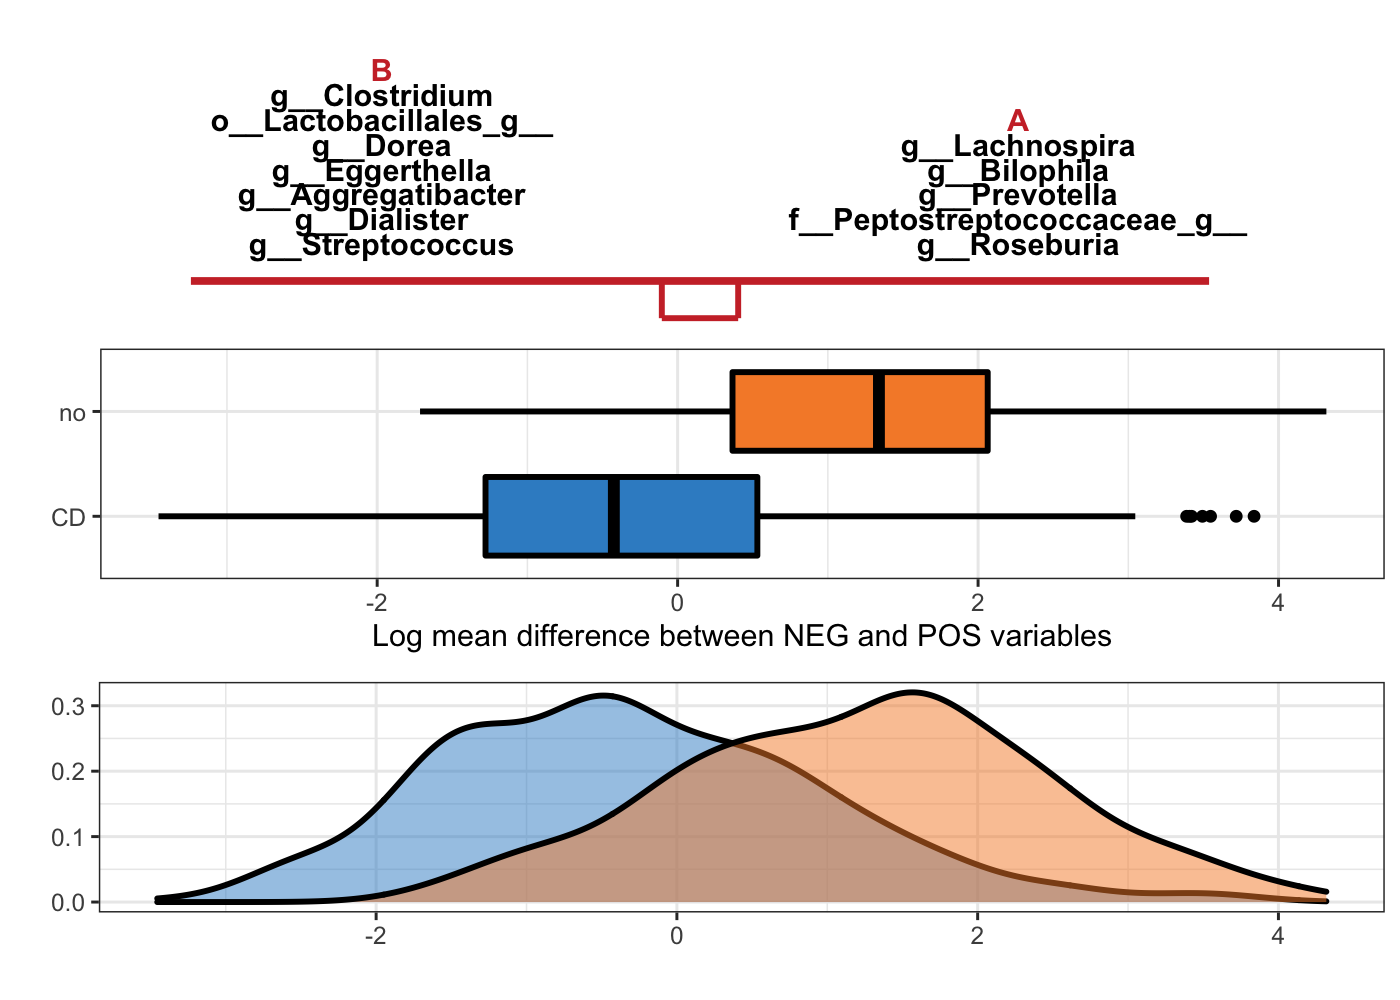
\includegraphics[width=1\linewidth]{./Generated_plots/codaCD-1} 

}

\caption{Selbal-like plot showing variables selected with method coda-lasso and the ability of these variables to discriminate CD and non-CD individuals.}\label{fig:codaCD}
\end{figure}

The interpretation of Figure \ref{fig:codaCD} is the same as Figure
\ref{fig:clrCD}, but with variables selected with method
\emph{coda-lasso}.

\subsection{plotLoadings}\label{plotloadings}

An easy way to visualise the coefficients of the selected variables is
to plot them in a barplot in \emph{mixMC} \citep{rohart2017mint}. We
have amended the \emph{plotLoadings()} function from the package
\emph{mixOmics} to do so. The argument \textbf{Y} specified the sample
class, so that the color assigened to each variable represents the class
that has the larger mean value (\textbf{method = `mean'} and
\textbf{contrib.method = `max'}).

\begin{Shaded}
\begin{Highlighting}[]
\CommentTok{# clr_lasso}
\NormalTok{Crohn.clr_coef <-}\StringTok{ }\NormalTok{Crohn.results_clrlasso}\OperatorTok{$}\NormalTok{coefficientsSelect}
\NormalTok{Crohn.clr_data <-}\StringTok{ }\NormalTok{x_Crohn[ ,Crohn.results_clrlasso}\OperatorTok{$}\NormalTok{varSelect]}
\NormalTok{Crohn.clr.plotloadings <-}\StringTok{ }\KeywordTok{plotcoefficients}\NormalTok{(}\DataTypeTok{coef =}\NormalTok{ Crohn.clr_coef, }
                                  \DataTypeTok{data =}\NormalTok{ Crohn.clr_data, }
                                  \DataTypeTok{Y =}\NormalTok{ y_Crohn, }
                                  \DataTypeTok{method =} \StringTok{'mean'}\NormalTok{, }
                                  \DataTypeTok{contrib.method =} \StringTok{'max'}\NormalTok{,}
                                  \DataTypeTok{title =} \StringTok{'Coefficients of clr-lasso on Crohn data'}\NormalTok{)}
\end{Highlighting}
\end{Shaded}

\begin{figure}

{\centering 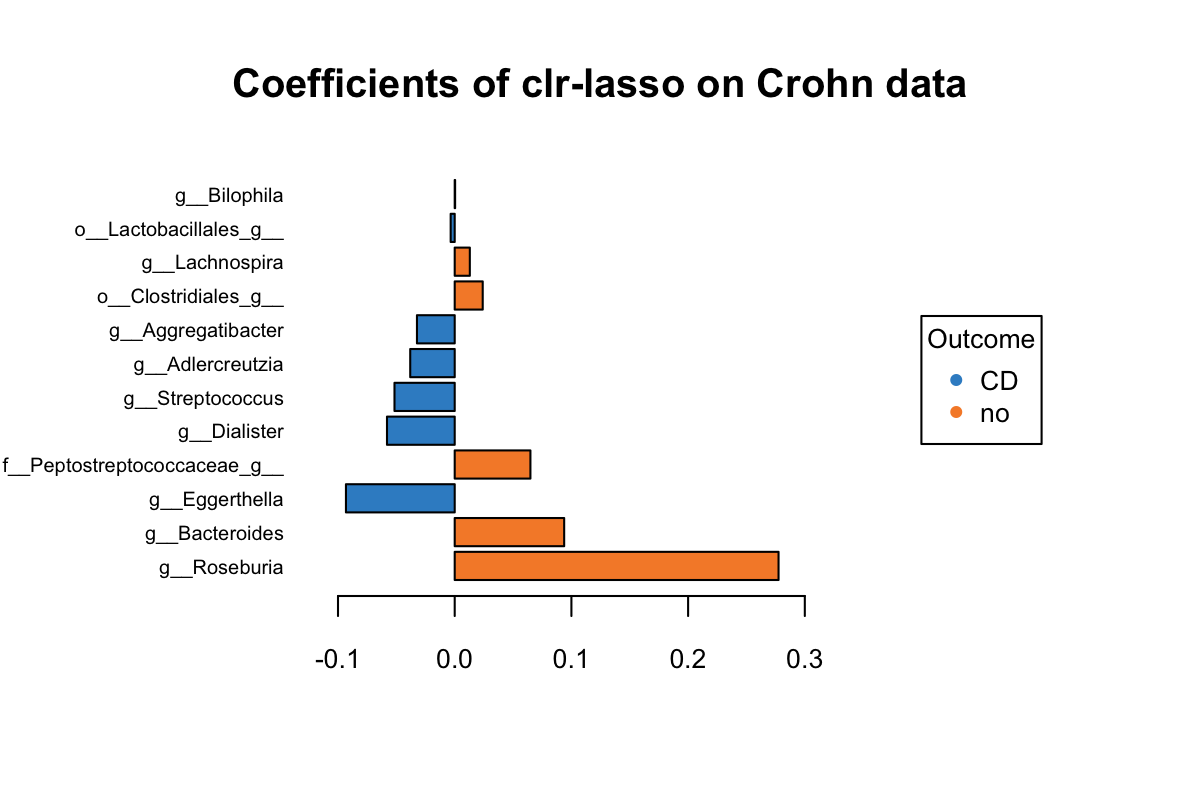
\includegraphics[width=1\linewidth]{./Generated_plots/loadclrCD-1} 

}

\caption{The plotLoadings of selected variables with clr-lasso.}\label{fig:loadclrCD}
\end{figure}

Figure \ref{fig:loadclrCD} shows that the variables colored in orange
have an abundance greater in non-CD samples relative to CD samples (e.g.
\emph{Roseburia}), while the blue ones have a greater abundance in CD
samples relative to non-CD samples (e.g. \emph{Eggerthella}). It is
based on their mean per group (CD vs.~non-CDs). The bar indicates the
coefficient. As we can see, all selected variables with a greater
abundance in non-CD samples have been assigned a positive coefficient,
and variables with a greater abundance in CD samples have been assigned
a negative coefficient.

\begin{Shaded}
\begin{Highlighting}[]
\CommentTok{# coda_lasso}
\NormalTok{Crohn.coda_coef <-}\StringTok{ }\NormalTok{Crohn.results_codalasso}\OperatorTok{$}\NormalTok{coefficientsSelect}
\NormalTok{Crohn.coda_data <-}\StringTok{ }\NormalTok{x_Crohn[ ,Crohn.results_codalasso}\OperatorTok{$}\NormalTok{varSelect]}

\NormalTok{Crohn.coda.plotloadings <-}\StringTok{ }\KeywordTok{plotcoefficients}\NormalTok{(}\DataTypeTok{coef =}\NormalTok{ Crohn.coda_coef, }
                                \DataTypeTok{data =}\NormalTok{ Crohn.coda_data, }
                                \DataTypeTok{Y =}\NormalTok{ y_Crohn, }
                                \DataTypeTok{method =} \StringTok{'mean'}\NormalTok{, }
                                \DataTypeTok{contrib.method =} \StringTok{'max'}\NormalTok{,}
                                \DataTypeTok{title =} \StringTok{'Coefficients of coda-lasso on Crohn data'}\NormalTok{)}
\end{Highlighting}
\end{Shaded}

\begin{figure}

{\centering 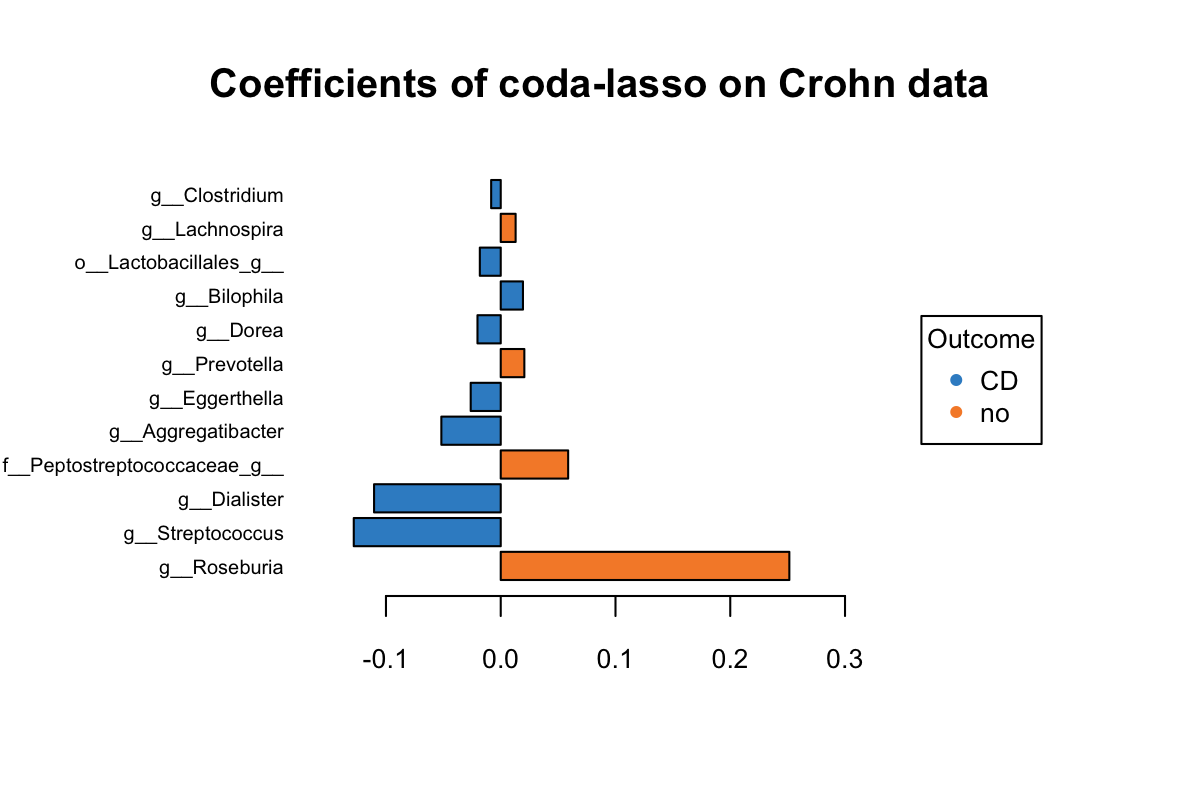
\includegraphics[width=1\linewidth]{./Generated_plots/loadcodaCD-1} 

}

\caption{The plotLoadings of selected variables with coda-lasso.}\label{fig:loadcodaCD}
\end{figure}

The same as Figure \ref{fig:loadclrCD}, we can interpret Figure
\ref{fig:loadcodaCD} as follows. Both \emph{Roseburia} and
\emph{Peptostreptococcaceae} selected by \emph{clr-lasso} and
\emph{coda-lasso} have a greater abundance in non-CD group and were
assigned with the same coeffcient rank. But both \emph{Eggerthella} and
\emph{Dialister} selected by two methods were assigned with very
different coefficient rank. Several variables have a greater abundance
in CD group, but with a positive coefficient. It means this model is not
optimal at some extent. This may suggest that \emph{clr-lasso} is better
at identifying discriminative variables than \emph{coda-lasso}.

\subsection{Trajectory plots}\label{trajectory-plots}

To visualise the change of variable coefficients and their ranks in the
selection between different methods, we use \emph{trajectory plots}.

\begin{Shaded}
\begin{Highlighting}[]
\KeywordTok{TRAJ_plot}\NormalTok{(}\DataTypeTok{selectVar_coef_method1 =}\NormalTok{ Crohn.coda_coef, }
          \DataTypeTok{selectVar_coef_method2 =}\NormalTok{ Crohn.clr_coef, }
          \DataTypeTok{selectMethods =} \KeywordTok{c}\NormalTok{(}\StringTok{'coda-lasso'}\NormalTok{, }\StringTok{'clr-lasso'}\NormalTok{))}
\end{Highlighting}
\end{Shaded}

\begin{figure}

{\centering 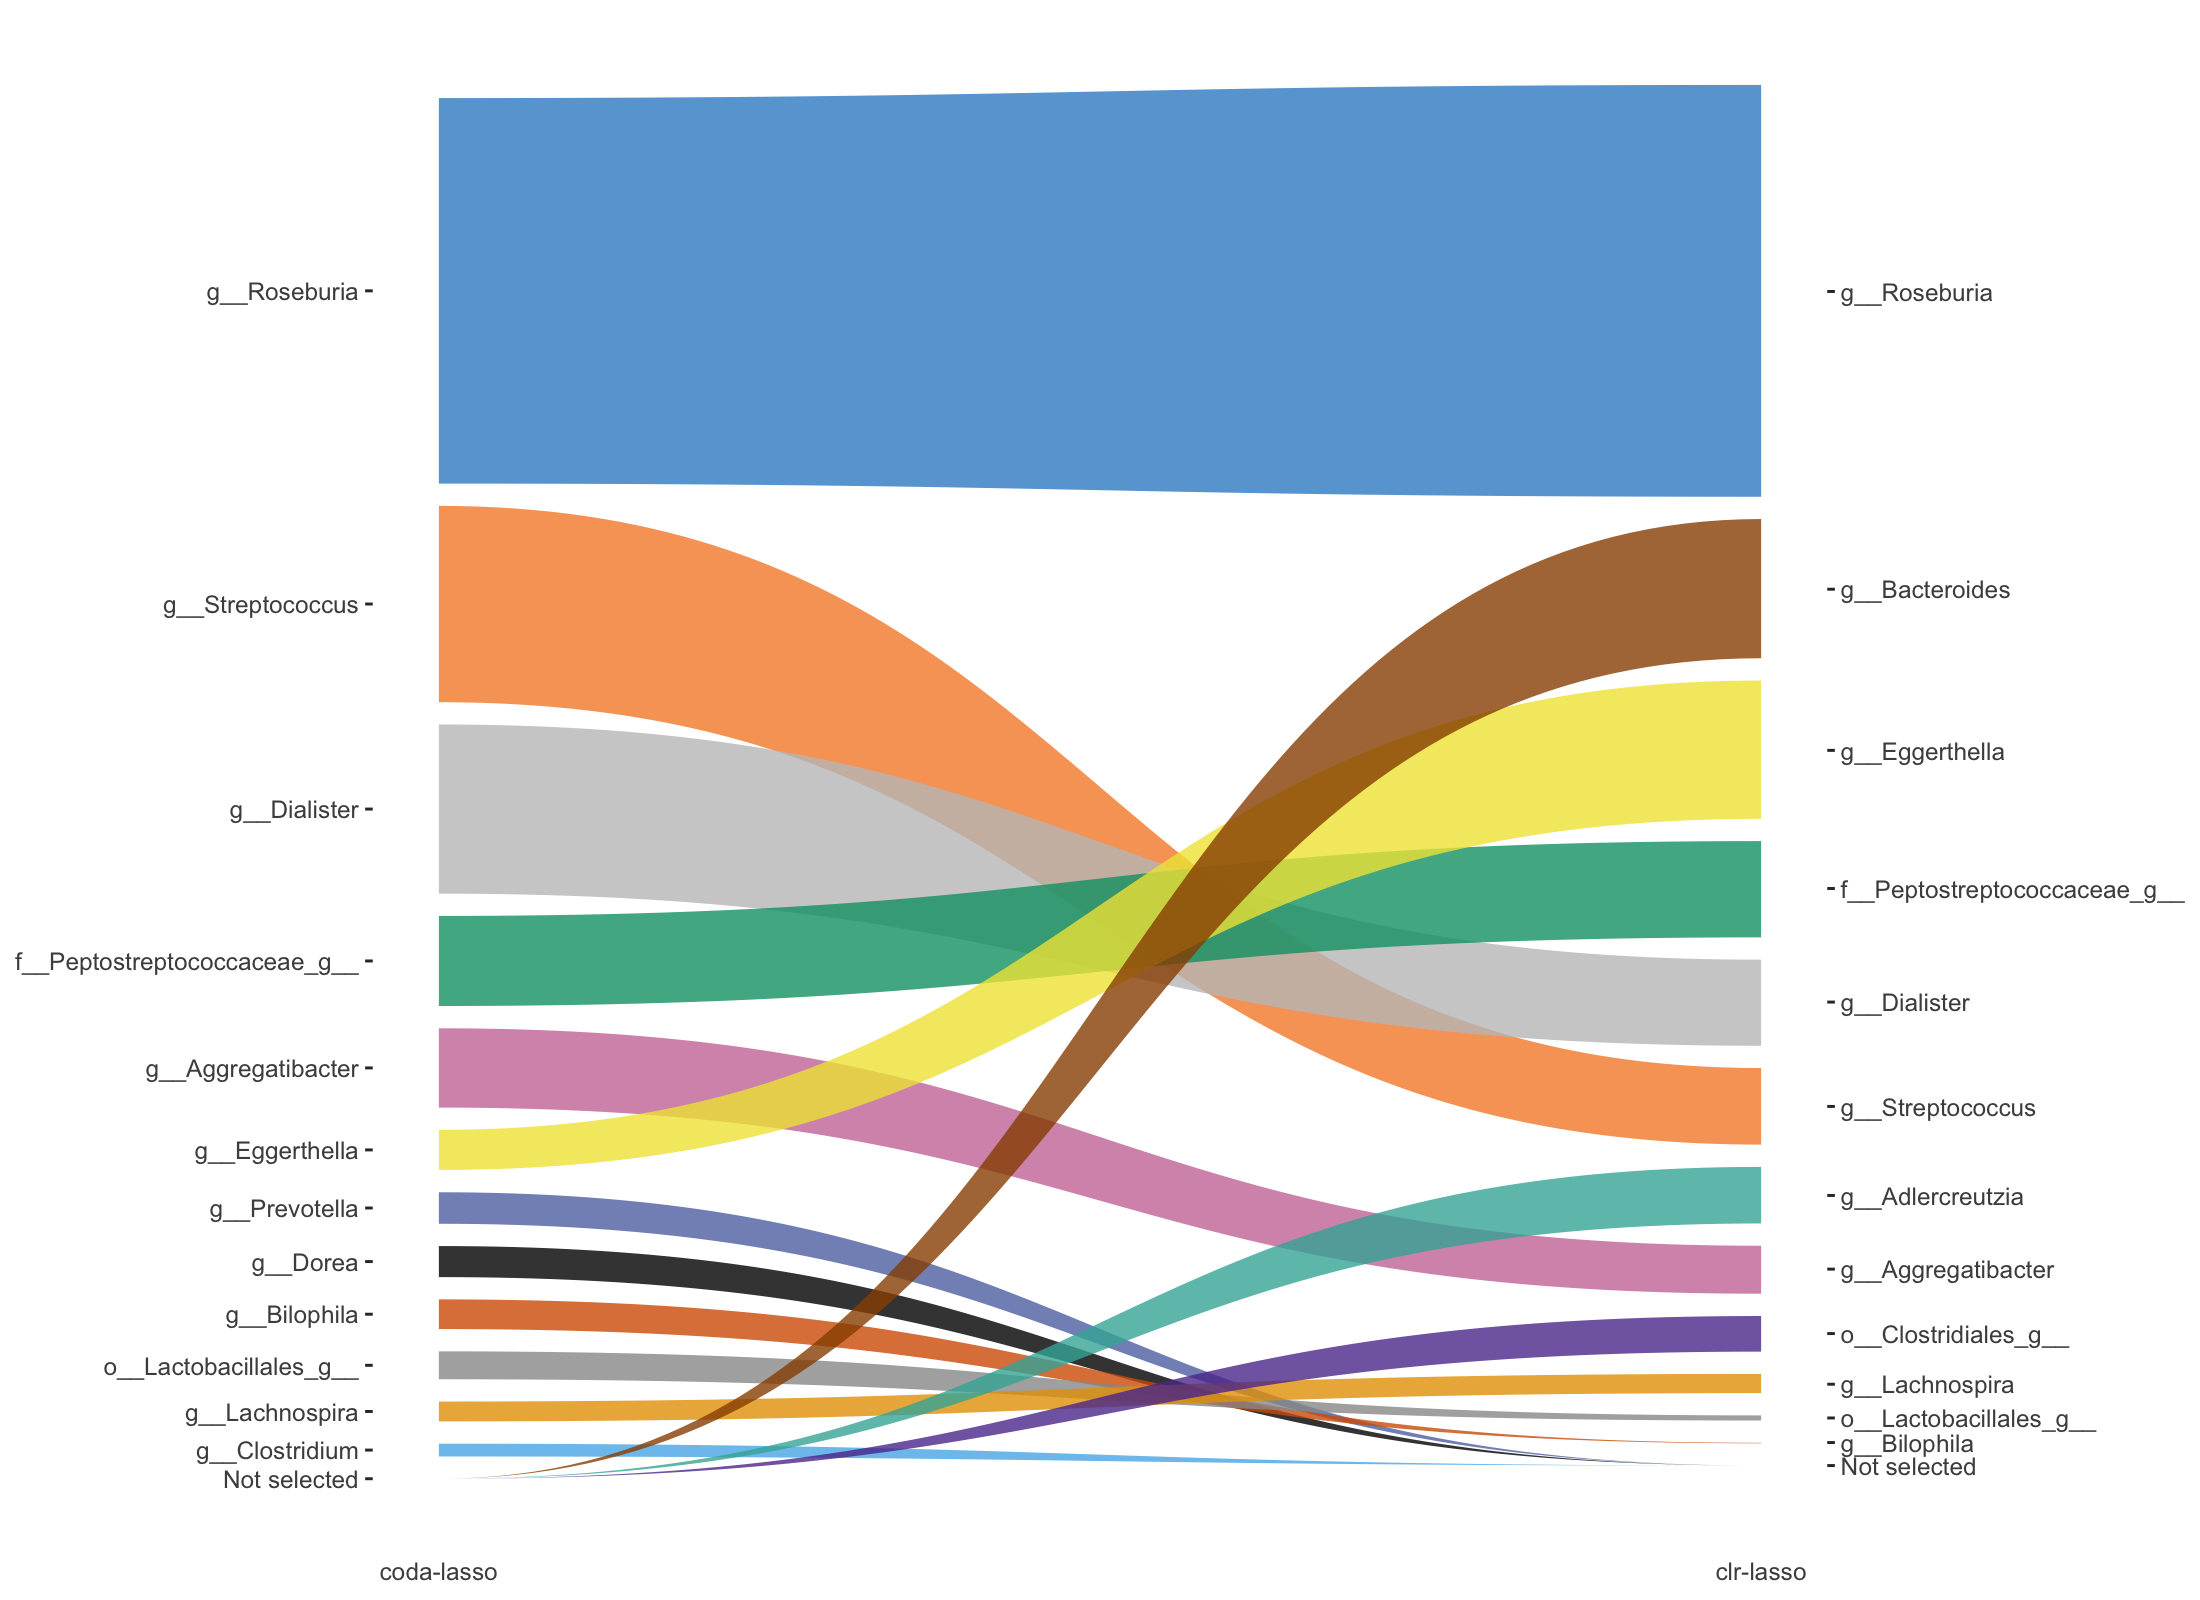
\includegraphics[width=1\linewidth]{./Generated_plots/trajCD-1} 

}

\caption{Trajectory plots of selected variables from both coda-lasso and clr-lasso in Crohn data.}\label{fig:trajCD}
\end{figure}

Figure \ref{fig:trajCD} shows the selected variables ordered by their
rank in the selection (according to their coefficient absolute values)
between \emph{coda-lasso} and \emph{clr-lasso}, with the thickness of
the lines representing the coefficient absolute values.

In this plot \ref{fig:trajCD}, we can visualise the rank change of each
selected variable between \emph{coda-lasso} and \emph{clr-lasso}
selection. For example, the rank of \emph{Dialister} is lower in
\emph{clr-lasso} compared to \emph{coda-lasso}. Moreover, we can detect
the variables (e.g. \emph{Bacteroides}) that are selected by one method
(e.g. \emph{clr-lasso}) with high coefficient rank, but not selected by
the other method (e.g. \emph{coda-lasso}).

\section{HFHS-Day1 case study}\label{hfhs-day1-case-study-3}

Guidance on how to interpret the following plots is detailed in previous
\textbf{section: Crohn case study}.

\subsection{UpSetR}\label{upsetr-1}

\begin{Shaded}
\begin{Highlighting}[]
\NormalTok{HFHS.select <-}\StringTok{ }\KeywordTok{list}\NormalTok{(}\DataTypeTok{selbal =}\NormalTok{ HFHS.results_selbal}\OperatorTok{$}\NormalTok{varSelect,}
                    \DataTypeTok{clr_lasso =}\NormalTok{ HFHS.results_clrlasso}\OperatorTok{$}\NormalTok{varSelect,}
                    \DataTypeTok{coda_lasso =}\NormalTok{ HFHS.results_codalasso}\OperatorTok{$}\NormalTok{varSelect)}

\NormalTok{HFHS.select.upsetR <-}\StringTok{ }\KeywordTok{fromList}\NormalTok{(HFHS.select)}

\KeywordTok{upset}\NormalTok{(}\KeywordTok{as.data.frame}\NormalTok{(HFHS.select.upsetR), }\DataTypeTok{main.bar.color =} \StringTok{'gray36'}\NormalTok{, }
      \DataTypeTok{sets.bar.color =}\NormalTok{ color[}\KeywordTok{c}\NormalTok{(}\DecValTok{1}\NormalTok{,}\DecValTok{2}\NormalTok{,}\DecValTok{5}\NormalTok{)], }\DataTypeTok{matrix.color =} \StringTok{'gray36'}\NormalTok{, }
      \DataTypeTok{order.by =} \StringTok{'freq'}\NormalTok{, }\DataTypeTok{empty.intersections =} \StringTok{'on'}\NormalTok{, }
      \DataTypeTok{queries =} \KeywordTok{list}\NormalTok{(}\KeywordTok{list}\NormalTok{(}\DataTypeTok{query =}\NormalTok{ intersects, }\DataTypeTok{params =} \KeywordTok{list}\NormalTok{(}\StringTok{'selbal'}\NormalTok{), }
                          \DataTypeTok{color =}\NormalTok{ color[}\DecValTok{5}\NormalTok{], }\DataTypeTok{active =}\NormalTok{ T), }
                     \KeywordTok{list}\NormalTok{(}\DataTypeTok{query =}\NormalTok{ intersects, }\DataTypeTok{params =} \KeywordTok{list}\NormalTok{(}\StringTok{'coda_lasso'}\NormalTok{), }
                          \DataTypeTok{color =}\NormalTok{ color[}\DecValTok{2}\NormalTok{], }\DataTypeTok{active =}\NormalTok{ T),}
                     \KeywordTok{list}\NormalTok{(}\DataTypeTok{query =}\NormalTok{ intersects, }\DataTypeTok{params =} \KeywordTok{list}\NormalTok{(}\StringTok{'clr_lasso'}\NormalTok{), }
                          \DataTypeTok{color =}\NormalTok{ color[}\DecValTok{1}\NormalTok{], }\DataTypeTok{active =}\NormalTok{ T)))}
\end{Highlighting}
\end{Shaded}

\begin{figure}

{\centering 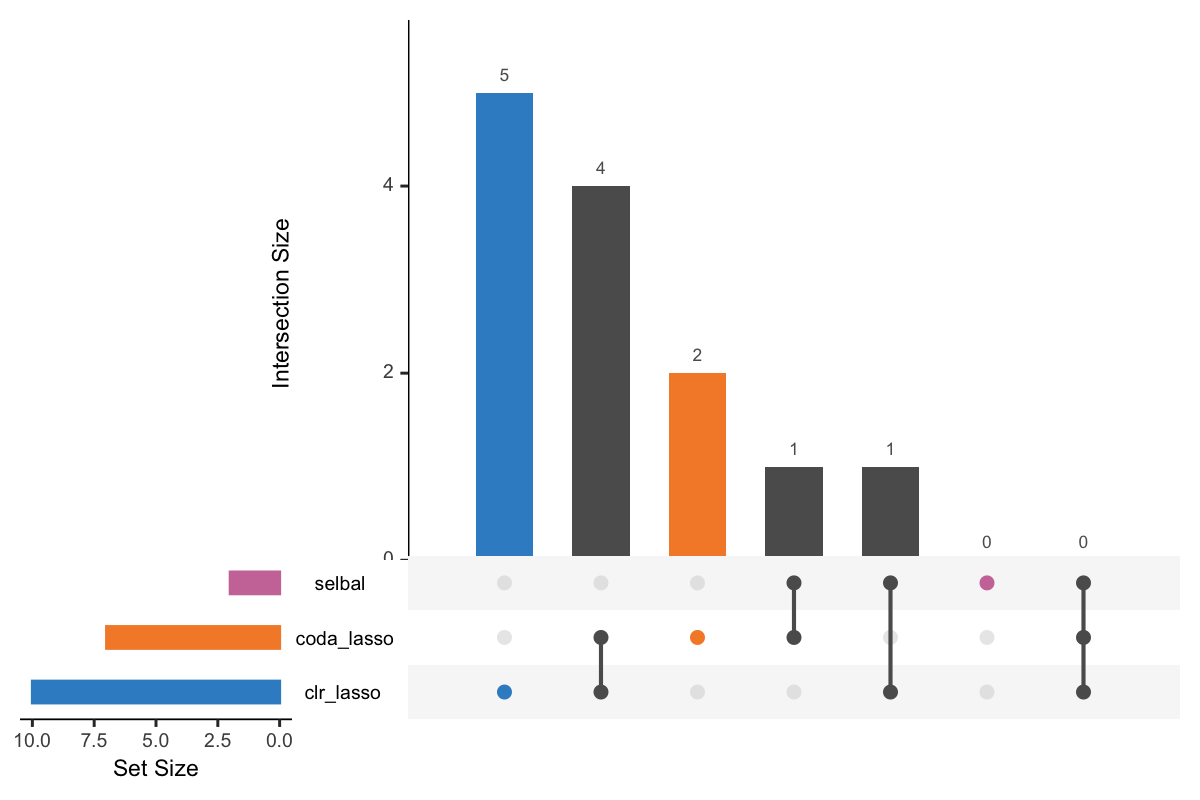
\includegraphics[width=1\linewidth]{./Generated_plots/upsetHFHS-1} 

}

\caption{UpSet plot showing overlap between variables selected with different methods.}\label{fig:upsetHFHS}
\end{figure}

Figure \ref{fig:upsetHFHS} shows that 5 OTUs are only selected with
\emph{clr-lasso}, 4 OTUs are selected both with \emph{coda-lasso} and
\emph{clr-lasso}, 2 OTUs are only selected with \emph{coda-lasso}, 1
OTUs is selected with both \emph{selbal} and \emph{coda-lasso}, and 1 is
selected both with \emph{selbal} and \emph{clr-lasso}. Among three
methods, \emph{clr-lasso} selected the largest number of OTUs and
\emph{selbal} the smallest.

\subsection{Selbal-like plot}\label{selbal-like-plot-1}

\begin{Shaded}
\begin{Highlighting}[]
\CommentTok{# selbal}
\NormalTok{HFHS.selbal_pos <-}\StringTok{ }\NormalTok{HFHS.results_selbal}\OperatorTok{$}\NormalTok{posVarSelect}
\NormalTok{HFHS.selbal_neg <-}\StringTok{ }\NormalTok{HFHS.results_selbal}\OperatorTok{$}\NormalTok{negVarSelect}
\KeywordTok{selbal_like_plot}\NormalTok{(}\DataTypeTok{pos.names =}\NormalTok{ HFHS.selbal_pos, }
                 \DataTypeTok{neg.names =}\NormalTok{ HFHS.selbal_neg, }
                 \DataTypeTok{Y =}\NormalTok{ y_HFHSday1, }\DataTypeTok{selbal =} \OtherTok{TRUE}\NormalTok{, }
                 \DataTypeTok{FINAL.BAL =}\NormalTok{ HFHS.results_selbal}\OperatorTok{$}\NormalTok{finalBal, }
                 \DataTypeTok{OTU =}\NormalTok{ T, }\DataTypeTok{taxa =}\NormalTok{ taxonomy_HFHS)}
\end{Highlighting}
\end{Shaded}

\begin{figure}

{\centering 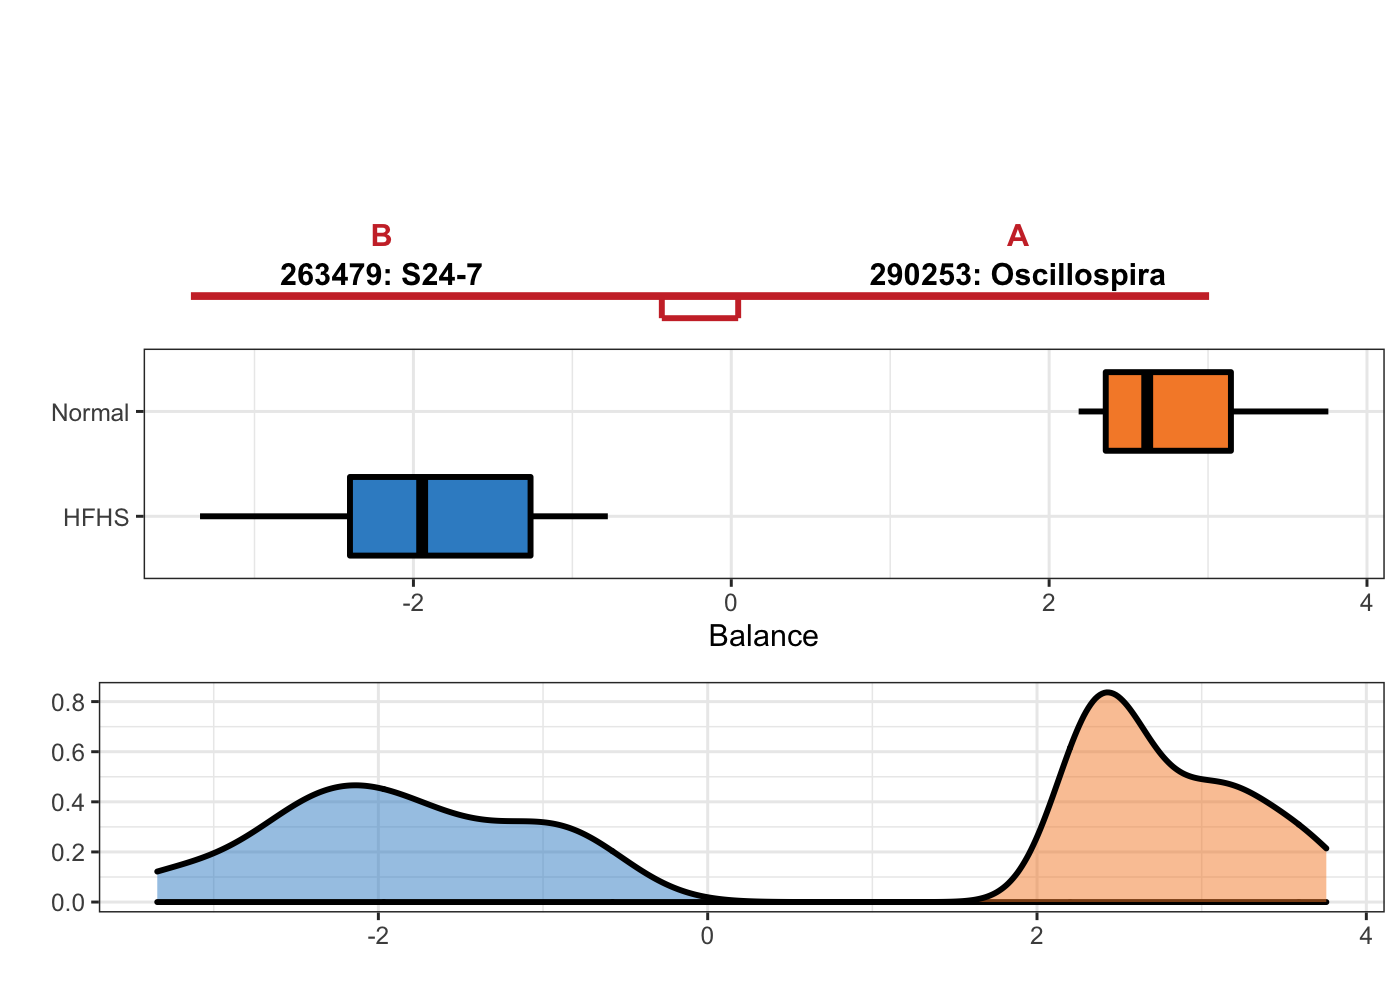
\includegraphics[width=1\linewidth]{./Generated_plots/unnamed-chunk-52-1} 

}

\caption{Selbal plot showing variables selected with methd selbal and the ability of these variables to discriminate HFHS and normal individuals.}\label{fig:unnamed-chunk-52}
\end{figure}

\begin{Shaded}
\begin{Highlighting}[]
\CommentTok{# clr_lasso}
\NormalTok{HFHS.clr_pos <-}\StringTok{ }\NormalTok{HFHS.results_clrlasso}\OperatorTok{$}\NormalTok{posCoefSelect}
\NormalTok{HFHS.clr_neg <-}\StringTok{ }\NormalTok{HFHS.results_clrlasso}\OperatorTok{$}\NormalTok{negCoefSelect}
\KeywordTok{selbal_like_plot}\NormalTok{(}\DataTypeTok{pos.names =} \KeywordTok{names}\NormalTok{(HFHS.clr_pos), }
                 \DataTypeTok{neg.names =} \KeywordTok{names}\NormalTok{(HFHS.clr_neg), }
                 \DataTypeTok{Y =}\NormalTok{ y_HFHSday1, }\DataTypeTok{X =}\NormalTok{ x_HFHSday1, }\DataTypeTok{OTU =}\NormalTok{ T, }
                 \DataTypeTok{taxa =}\NormalTok{ taxonomy_HFHS)}
\end{Highlighting}
\end{Shaded}

\begin{figure}

{\centering 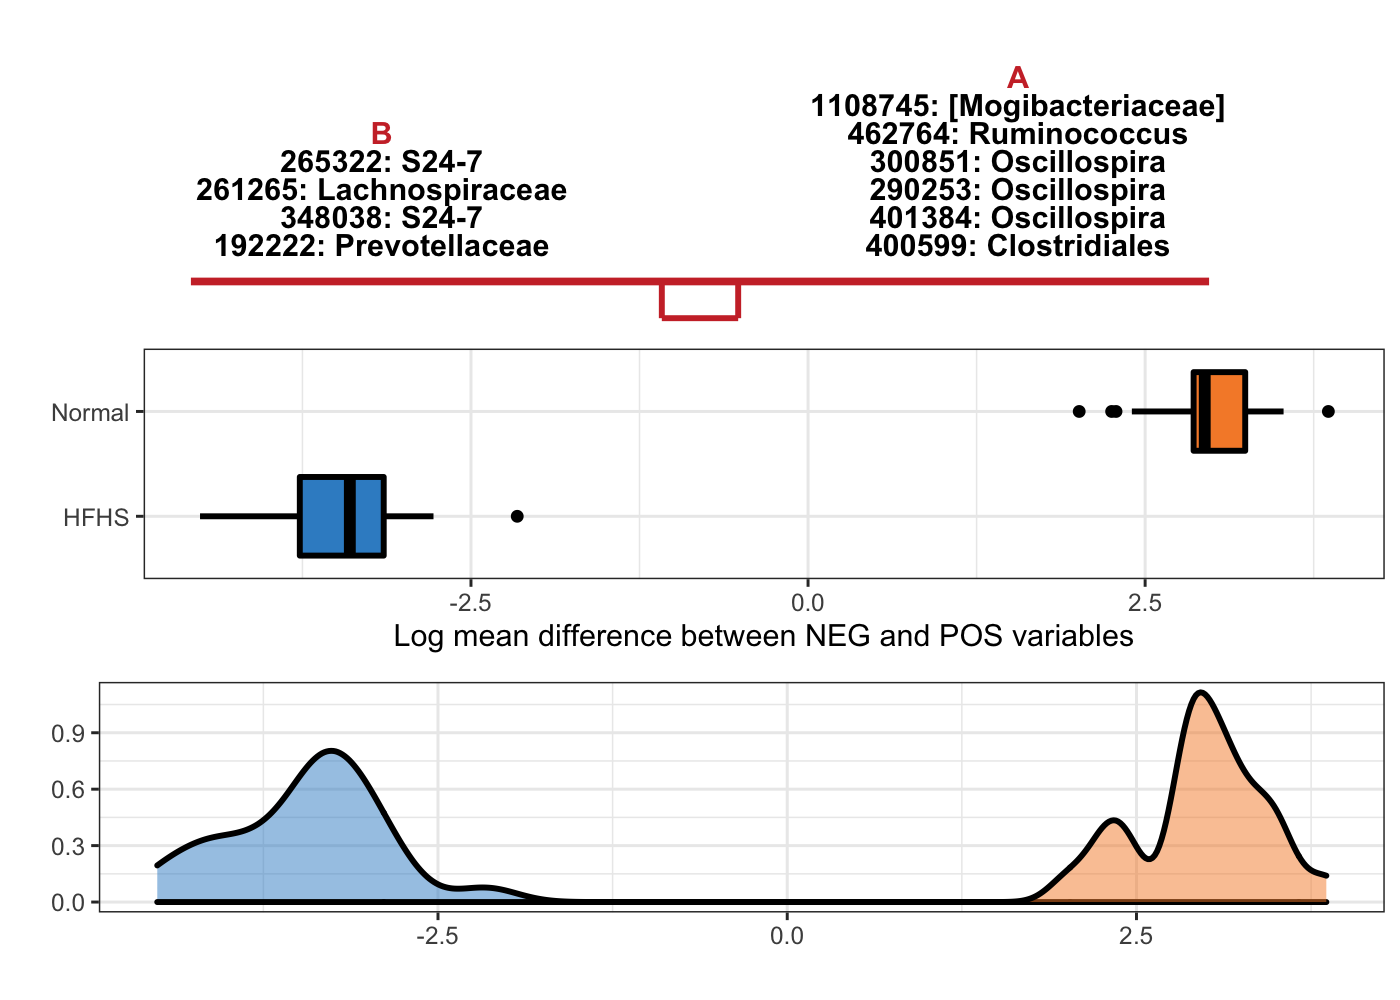
\includegraphics[width=1\linewidth]{./Generated_plots/unnamed-chunk-53-1} 

}

\caption{Selbal-like plot showing variables selected with method clr-lasso and the ability of these variables to discriminate HFHS and normal individuals.}\label{fig:unnamed-chunk-53}
\end{figure}

\begin{Shaded}
\begin{Highlighting}[]
\CommentTok{# coda_lasso}
\NormalTok{HFHS.coda_pos <-}\StringTok{ }\NormalTok{HFHS.results_codalasso}\OperatorTok{$}\NormalTok{posCoefSelect}
\NormalTok{HFHS.coda_neg <-}\StringTok{ }\NormalTok{HFHS.results_codalasso}\OperatorTok{$}\NormalTok{negCoefSelect}
\KeywordTok{selbal_like_plot}\NormalTok{(}\DataTypeTok{pos.names =} \KeywordTok{names}\NormalTok{(HFHS.coda_pos), }
                 \DataTypeTok{neg.names =} \KeywordTok{names}\NormalTok{(HFHS.coda_neg), }
                 \DataTypeTok{Y =}\NormalTok{ y_HFHSday1, }\DataTypeTok{X =}\NormalTok{ x_HFHSday1, }
                 \DataTypeTok{OTU =}\NormalTok{ T, }\DataTypeTok{taxa =}\NormalTok{ taxonomy_HFHS)}
\end{Highlighting}
\end{Shaded}

\begin{figure}

{\centering 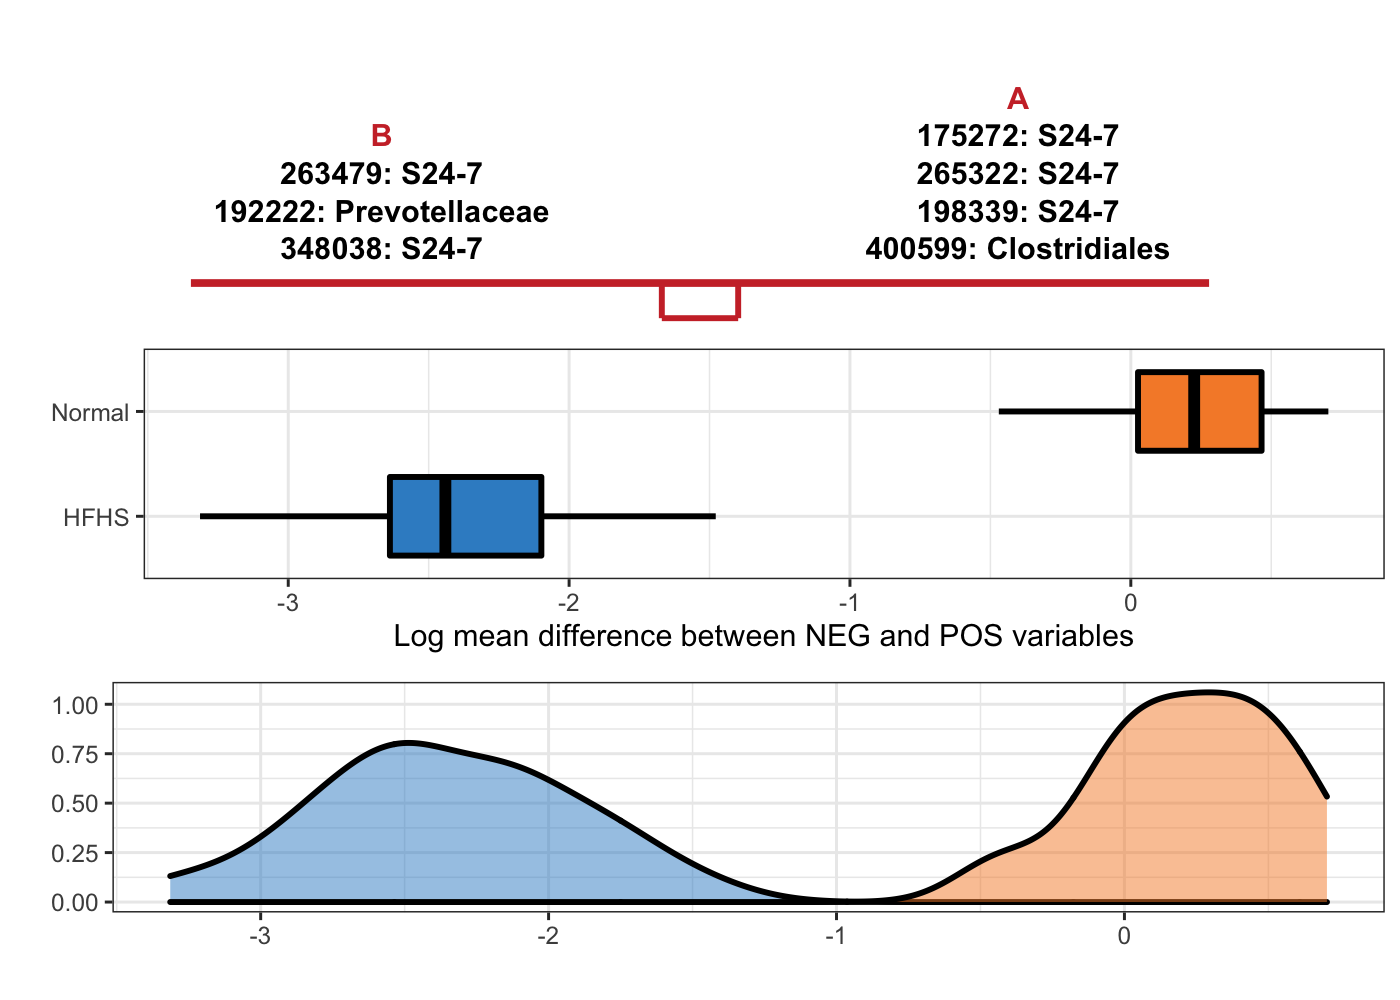
\includegraphics[width=1\linewidth]{./Generated_plots/unnamed-chunk-54-1} 

}

\caption{Selbal-like plot showing variables selected with method coda-lasso and the ability of these variables to discriminate HFHS and normal individuals.}\label{fig:unnamed-chunk-54}
\end{figure}

\emph{Note}: \emph{S24-7} is a family from order \emph{Bacteroidales}.

Among these methods, \emph{selbal} only needs two OTUs to build a
balance, it also means the association between microbiome composition
and diet is very strong.

\subsection{plotLoadings}\label{plotloadings-1}

\begin{Shaded}
\begin{Highlighting}[]
\CommentTok{# clr_lasso}
\NormalTok{HFHS.clr_coef <-}\StringTok{ }\NormalTok{HFHS.results_clrlasso}\OperatorTok{$}\NormalTok{coefficientsSelect}
\NormalTok{HFHS.clr_data <-}\StringTok{ }\NormalTok{x_HFHSday1[ ,HFHS.results_clrlasso}\OperatorTok{$}\NormalTok{varSelect]}
\NormalTok{HFHS.clr.plotloadings <-}\StringTok{ }\KeywordTok{plotcoefficients}\NormalTok{(}\DataTypeTok{coef =}\NormalTok{ HFHS.clr_coef, }
                              \DataTypeTok{data =}\NormalTok{ HFHS.clr_data, }
                              \DataTypeTok{Y =}\NormalTok{ y_HFHSday1, }
                              \DataTypeTok{title =} \StringTok{'Coefficients of clr-lasso on HFHS-Day1 data'}\NormalTok{,}
                              \DataTypeTok{method =} \StringTok{'mean'}\NormalTok{, }
                              \DataTypeTok{contrib.method =} \StringTok{'max'}\NormalTok{,}
                              \DataTypeTok{OTU =}\NormalTok{ T,}
                              \DataTypeTok{taxa =}\NormalTok{ taxonomy_HFHS)}
\end{Highlighting}
\end{Shaded}

\begin{figure}

{\centering 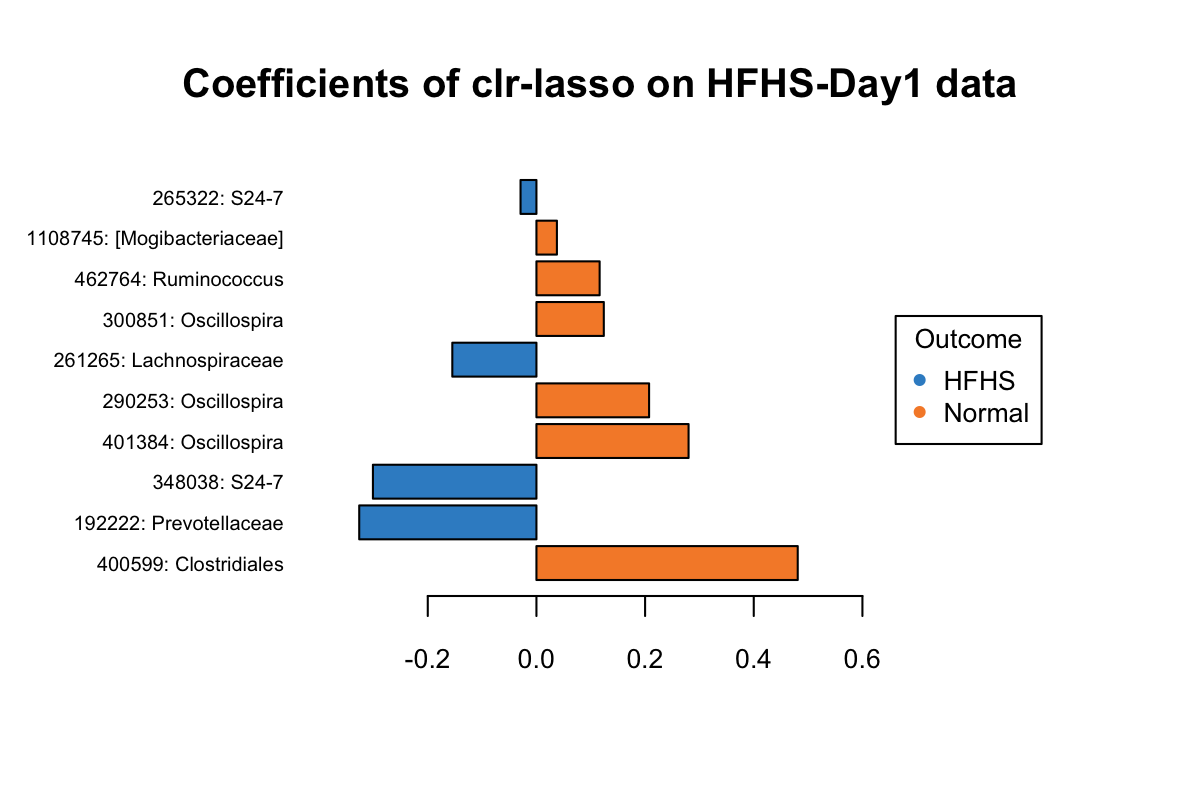
\includegraphics[width=1\linewidth]{./Generated_plots/loadclrHFHS-1} 

}

\caption{The plotLoadings of selected variables with clr-lasso.}\label{fig:loadclrHFHS}
\end{figure}

\begin{Shaded}
\begin{Highlighting}[]
\CommentTok{# coda_lasso}
\NormalTok{HFHS.coda_coef <-}\StringTok{ }\NormalTok{HFHS.results_codalasso}\OperatorTok{$}\NormalTok{coefficientsSelect}
\NormalTok{HFHS.coda_data <-}\StringTok{ }\NormalTok{x_HFHSday1[ ,HFHS.results_codalasso}\OperatorTok{$}\NormalTok{varSelect]}

\NormalTok{HFHS.coda.plotloadings <-}\StringTok{ }\KeywordTok{plotcoefficients}\NormalTok{(}\DataTypeTok{coef =}\NormalTok{ HFHS.coda_coef, }
                            \DataTypeTok{data =}\NormalTok{ HFHS.coda_data, }
                            \DataTypeTok{Y =}\NormalTok{ y_HFHSday1, }
                            \DataTypeTok{method =} \StringTok{'mean'}\NormalTok{, }
                            \DataTypeTok{contrib.method =} \StringTok{'max'}\NormalTok{,}
                            \DataTypeTok{title =} \StringTok{'Coefficients of coda-lasso on HFHS-Day1 data'}\NormalTok{,}
                            \DataTypeTok{OTU =}\NormalTok{ T,}
                            \DataTypeTok{taxa =}\NormalTok{ taxonomy_HFHS)}
\end{Highlighting}
\end{Shaded}

\begin{figure}

{\centering 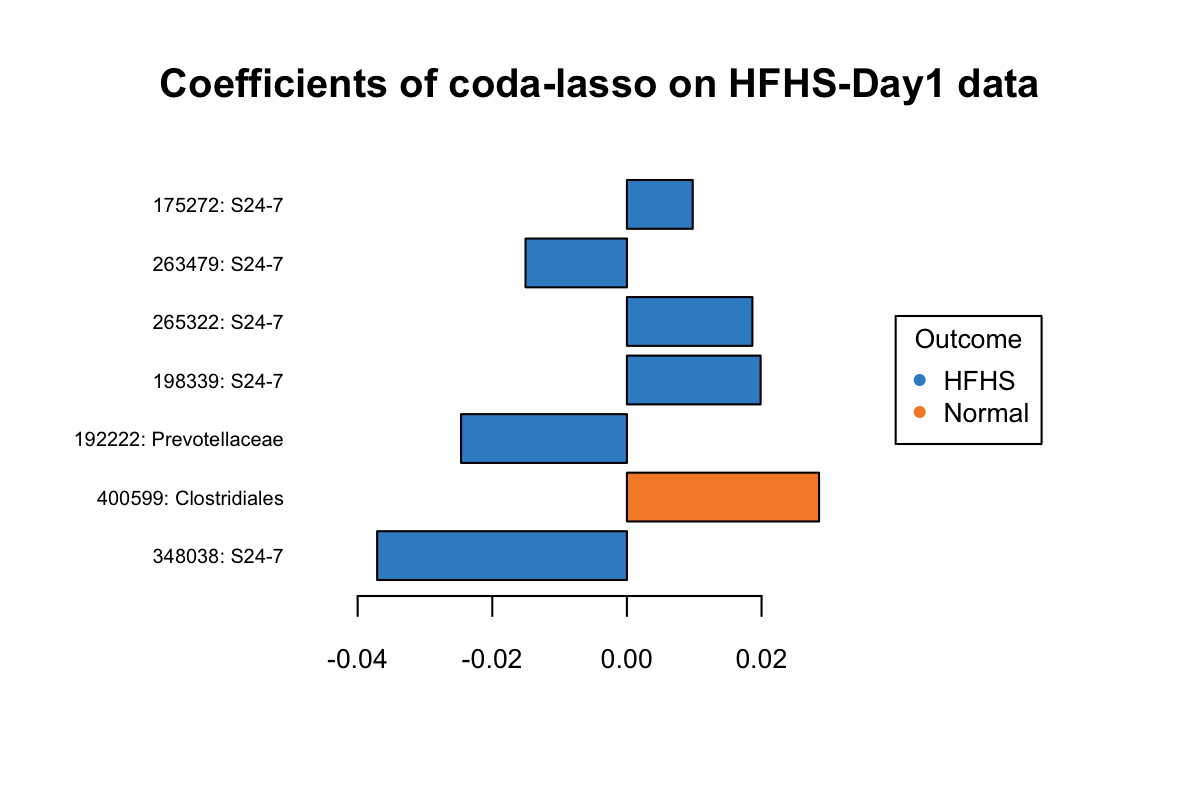
\includegraphics[width=1\linewidth]{./Generated_plots/loadcodaHFHS-1} 

}

\caption{The plotLoadings of selected variables with coda-lasso.}\label{fig:loadcodaHFHS}
\end{figure}

In Figure \ref{fig:loadcodaHFHS}, three OTUs \textbf{175272: S24-7},
\textbf{265322: S24-7}, \textbf{198339: S24-7} have a greater abundance
in HFHS group but were assigned with positive coefficients.

\subsection{Trajectory plots}\label{trajectory-plots-1}

\begin{Shaded}
\begin{Highlighting}[]
\KeywordTok{TRAJ_plot}\NormalTok{(}\DataTypeTok{selectVar_coef_method1 =}\NormalTok{ HFHS.coda_coef, }
          \DataTypeTok{selectVar_coef_method2 =}\NormalTok{ HFHS.clr_coef, }
          \DataTypeTok{selectMethods =} \KeywordTok{c}\NormalTok{(}\StringTok{'coda-lasso'}\NormalTok{, }\StringTok{'clr-lasso'}\NormalTok{), }
          \DataTypeTok{OTU =}\NormalTok{ T, }\DataTypeTok{taxa =}\NormalTok{ taxonomy_HFHS)}
\end{Highlighting}
\end{Shaded}

\begin{figure}

{\centering 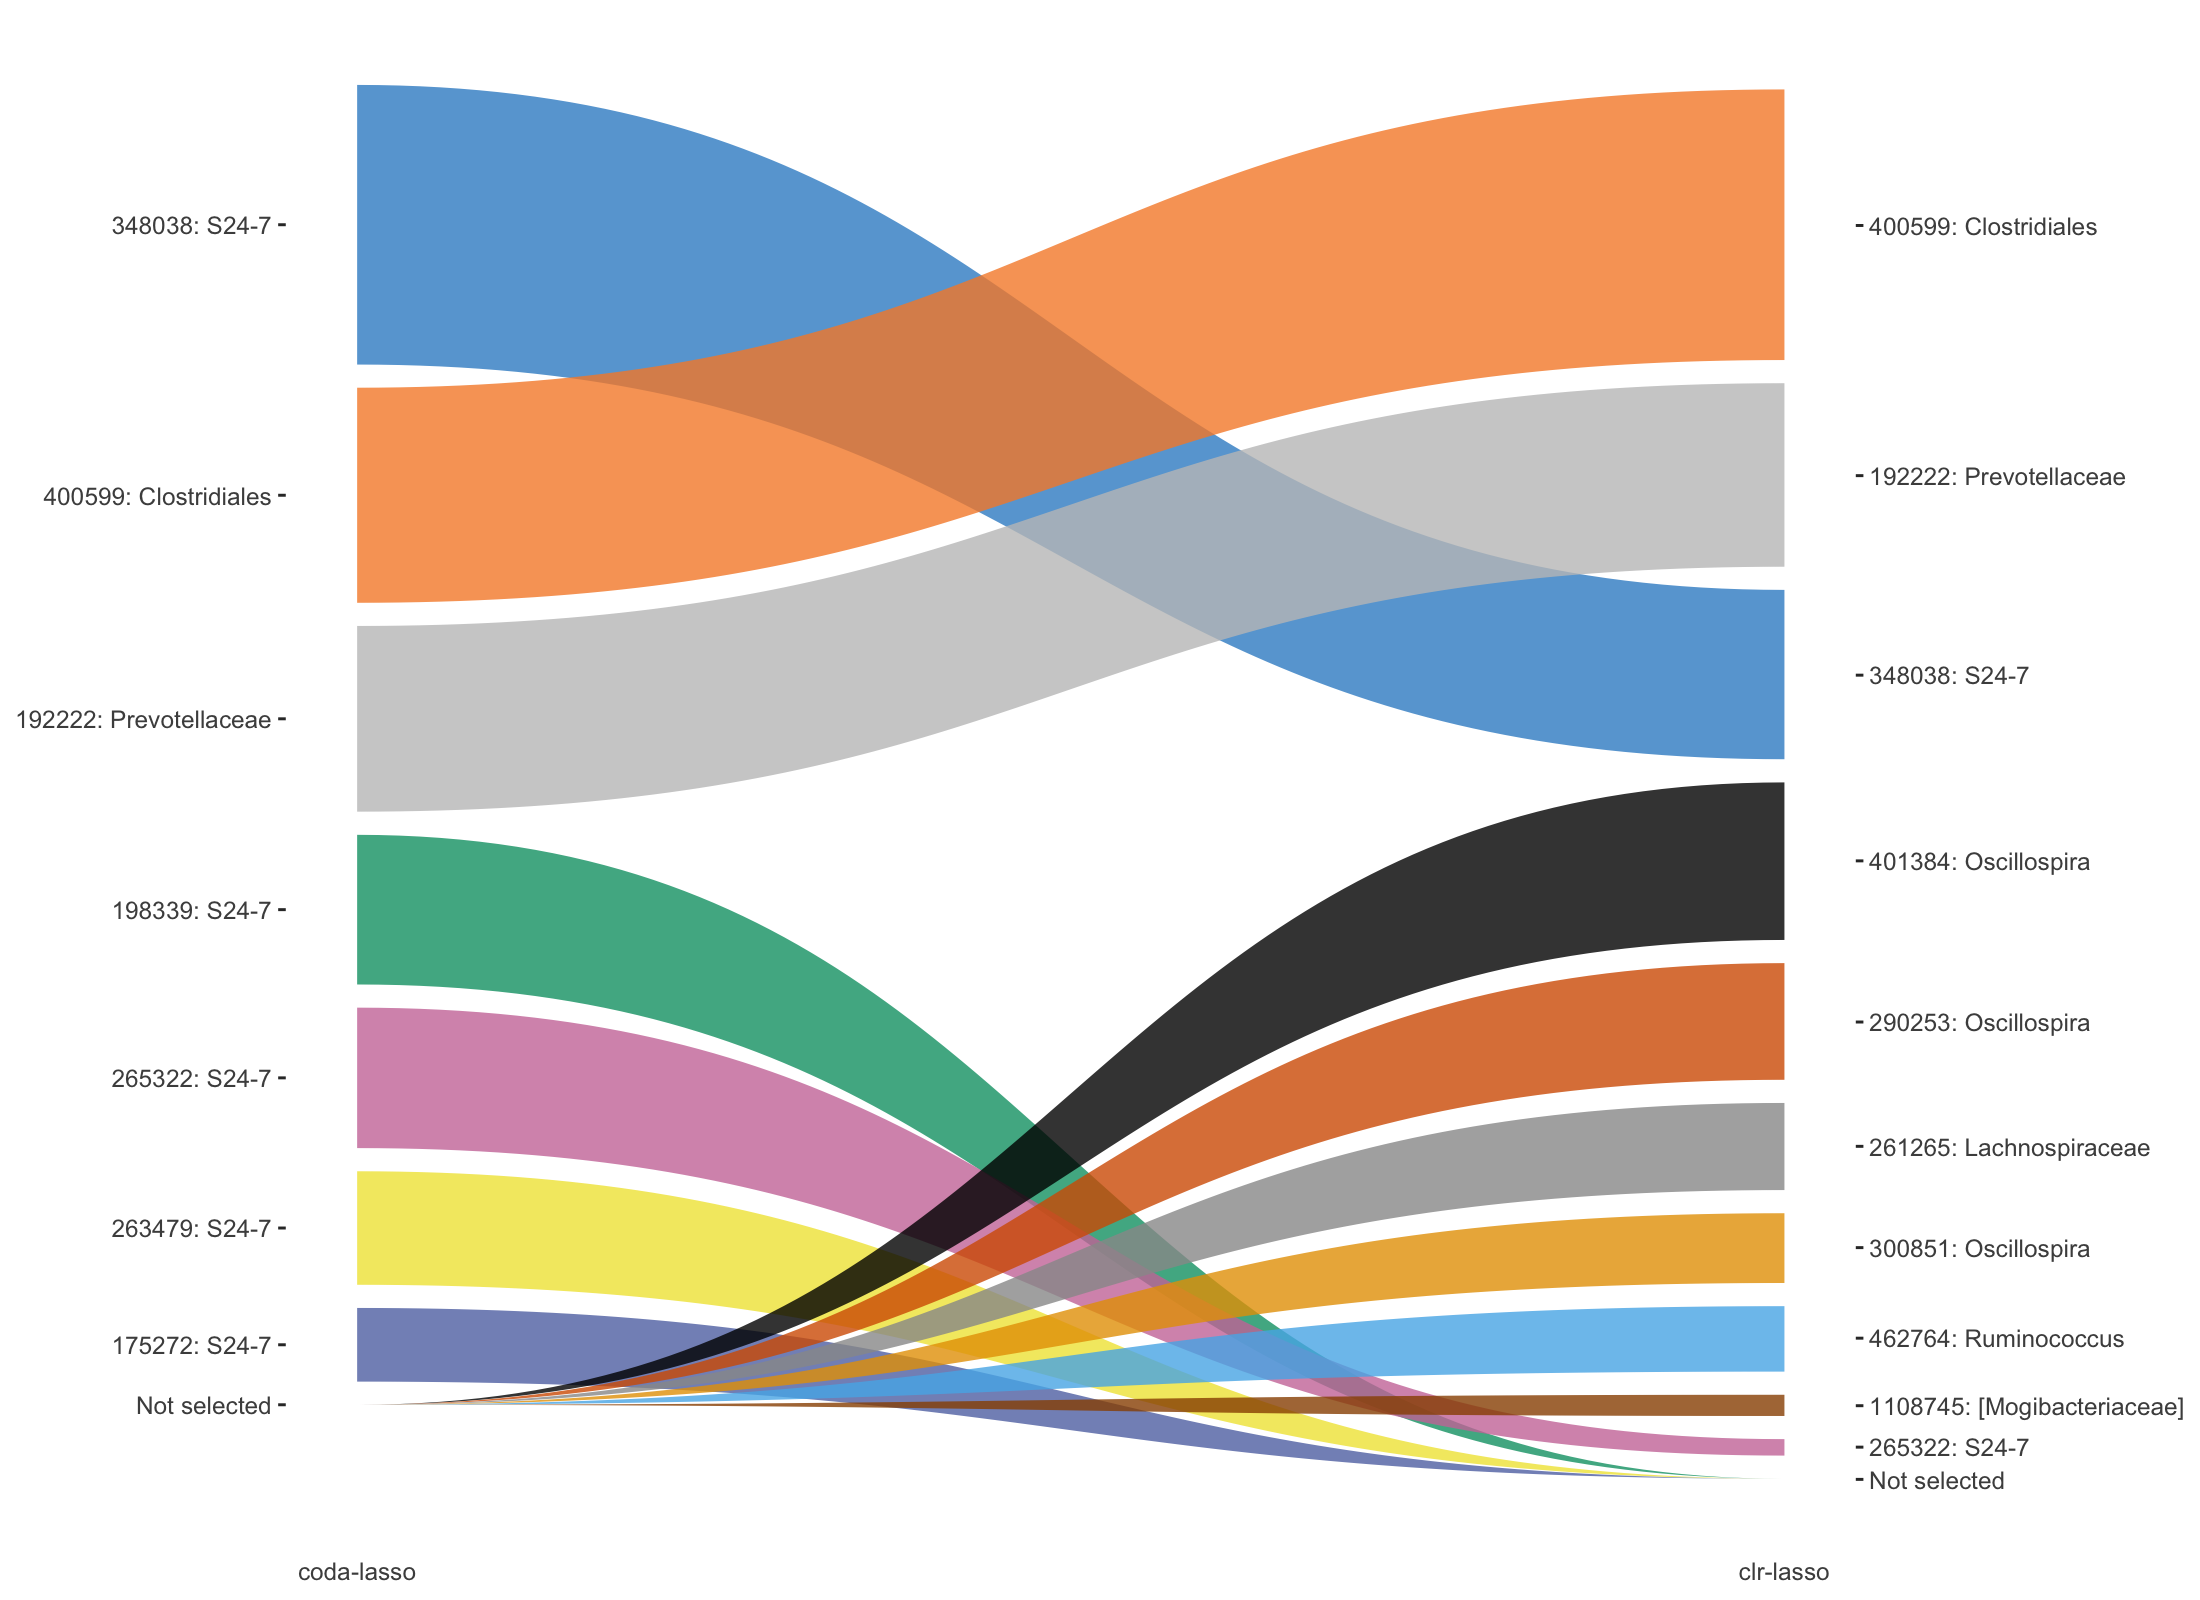
\includegraphics[width=1\linewidth]{./Generated_plots/trajHFHS-1} 

}

\caption{Trajectory plots of selected variables with both coda-lasso and clr-lasso in HFHSday1 data.}\label{fig:trajHFHS}
\end{figure}

In Figure \ref{fig:trajHFHS}, top three OTUs selected with
\emph{clr-lasso} are also selected as top OTUs from \emph{coda-lasso}
but with different order. The other OTUs are either selected by
\emph{coda-lasso} or \emph{clr-lasso}.

\subsection{GraPhlAn}\label{graphlan}

As we also have the taxonomic information of HFHSday1 data, we use
\emph{GraPhlAn} to visualise the taxonomic information of the selected
OTUs. \emph{GraPhlAn} is a software tool for producing high-quality
circular representations of taxonomic and phylogenetic trees
(\url{https://huttenhower.sph.harvard.edu/graphlan}). It is coded in
Python.

We first remove empty taxa (e.g.~species) and aggregate all these
selected variables into a list. Then we use function
\emph{graphlan\_annot\_generation()} to generate the input files that
graphlan python codes require. In the \textbf{save\_folder}, there are
two existing files: \textbf{annot\_0.txt} and \textbf{graphlan\_all.sh}.
After we generate our input files \textbf{taxa.txt} and
\textbf{annot\_all.txt}, we only need to run the
\emph{./graphlan\_all.sh} in the bash command line to generate the plot.

\begin{Shaded}
\begin{Highlighting}[]
\CommentTok{# remove empty columns}
\NormalTok{HFHS.tax_codalasso <-}\StringTok{ }\NormalTok{HFHS.tax_codalasso[,}\OperatorTok{-}\DecValTok{7}\NormalTok{] }
\NormalTok{HFHS.tax_clrlasso <-}\StringTok{ }\NormalTok{HFHS.tax_clrlasso[,}\OperatorTok{-}\DecValTok{7}\NormalTok{]}
\NormalTok{HFHS.tax_selbal <-}\StringTok{ }\NormalTok{HFHS.tax_selbal[,}\OperatorTok{-}\DecValTok{7}\NormalTok{]}

\NormalTok{HFHS.select.tax <-}\StringTok{ }\KeywordTok{list}\NormalTok{(}\DataTypeTok{selbal =}\NormalTok{ HFHS.tax_selbal,}
                        \DataTypeTok{clr_lasso =}\NormalTok{ HFHS.tax_clrlasso,}
                        \DataTypeTok{coda_lasso =}\NormalTok{ HFHS.tax_codalasso)}

\KeywordTok{graphlan_annot_generation}\NormalTok{(}\DataTypeTok{taxa_list =}\NormalTok{ HFHS.select.tax, }\DataTypeTok{save_folder =} \StringTok{'graphlan/'}\NormalTok{)}
\end{Highlighting}
\end{Shaded}

\begin{figure}

{\centering 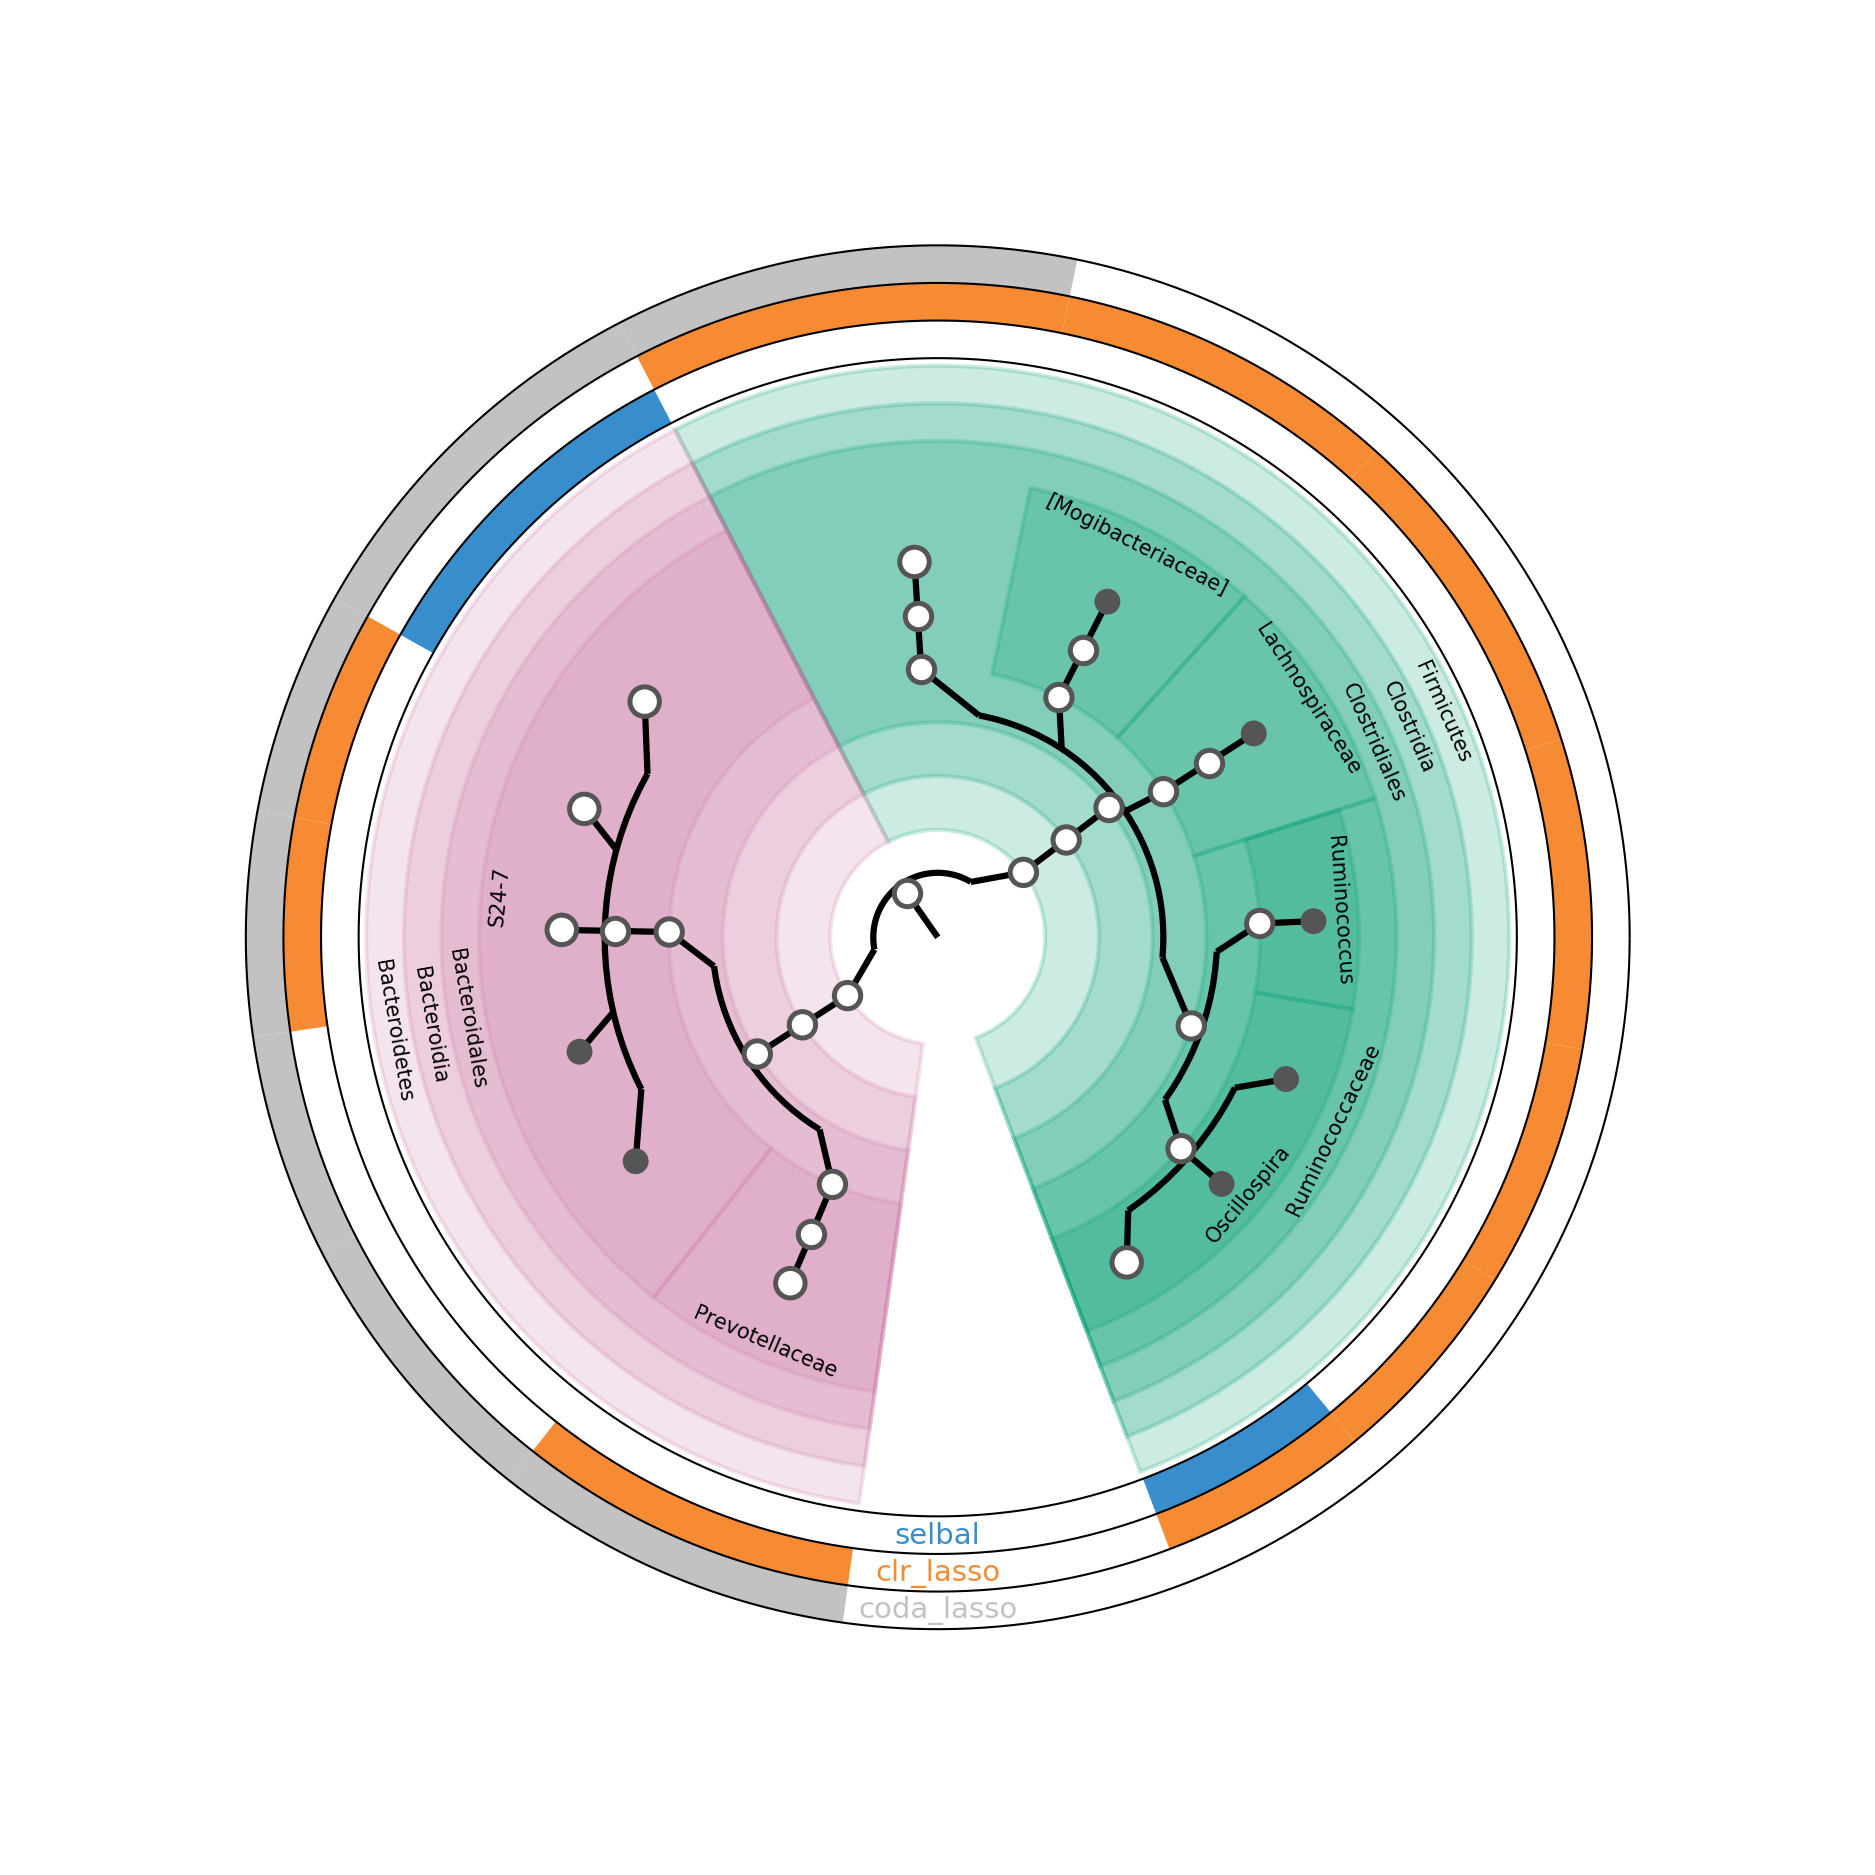
\includegraphics[width=1\linewidth]{./graphlan/taxa} 

}

\caption{GraPhlAn of selected taxa from different methods in HFHS-Day1 data.}\label{fig:graphlanHFHS}
\end{figure}

In Figure \ref{fig:graphlanHFHS}, the inner circle is a taxonomic tree
of selected OTUs. The outside circles indicate different selection
methods. If a proportion of a circle is coloured, it means that the
corresponding OTU is selected by the method labeled on the circle. If
the bottom nodes are coloured in gray, it indicates the OTUs are only
selected by one method.

\bibliography{book.bib}

\end{document}
